\documentclass[a4 paper, 12pt]{report}
\usepackage{hyperref}
\usepackage{apacite}
\usepackage{amssymb,dsfont,amsthm,amsmath,makeidx,verbatim,latexsym,amsfonts,mathrsfs}
\usepackage{cancel}
\setcounter{secnumdepth}{5}
\setcounter{tocdepth}{5}
\usepackage{graphicx}
\usepackage[none]{hyphenat}

\usepackage[english]{babel}
\addto{\captionsenglish}{%
	\renewcommand{\bibname}{REFERENCES}
	%\renewcommand{\tableofcontents}{Table of Contents}
}


\DeclareMathAlphabet{\mathpzc}{OT1}{pzc}{m}{it}
\newcommand*\rfrac[2]{{}^{#1}\!/_{#2}}

\hfuzz5pt
\theoremstyle{plain}
\newtheorem{theorem}{\textbf{Theorem}}[section]
\newtheorem{lemma}[theorem]{\textbf{Lemma}}
\newtheorem{proposition}[theorem]{\textbf{Proposition}}
\newtheorem{corollary}[theorem]{\textbf{Corollary}}
\newtheorem{claim}[theorem]{\textbf{Claim}}
\newtheorem{hypothesis}[theorem]{\textbf{Hypothesis}}
%\newtheorem{hypothesis}[theorem]{\textbf{Hypothesis}}
\newtheorem{definition}[theorem]{\textbf{Definition}}
\newtheorem{remark}[theorem]{\textbf{Remark}}
\newtheorem{example}[theorem]{\textbf{Example}}
\newtheorem{assumption}[theorem]{\textbf{Assumption}}
\newtheorem{notation}[theorem]{\textbf{Notation}}
\renewcommand{\baselinestretch}{1.50} % for the line spacing.
%spacing.
%\newcommand*\rfrac[2]{{}^{#1}\!/_{#2}}
\begin{document}
	\pagenumbering{roman} \baselineskip 29pt
\newcommand{\disp}{\displaystyle}
\thispagestyle{empty}


%\parindent 0pt
%\pagenumbering{roman}

%\begin{document}

\begin{center}
	\textbf{\large{APPROXIMATION OF SOLUTION OF STOCHASTIC FRACTIONAL DIFFERENTIAL EQUATIONS WITH NON-LIPSCHITZ  COEFFICIENTS}}
\end{center}
\ \
\begin{center}
	
	BY
\end{center}
\ \
\begin{center}
	\textbf{\large{ENWEREM, OLUCHI JANE}}
\end{center}
\begin{center}
	\textbf{Matric Number 217274}
\end{center}
\begin{center}
	Submitted to the Department of  Mathematics
\end{center}
\begin{center}
	Faculty of Science  
\end{center}
\begin{center}
	University of Ibadan, Ibadan,  
\end{center}
\begin{center}
	Nigeria  
\end{center}
\begin{center}
	In Partial Fulfillment of the Award of Master of Science in Mathematics
\end{center}
\begin{center}
	In the Department of Mathematics Faculty of Science
\end{center}
\begin{center}
	University of Ibadan, Ibadan,  
\end{center}
\begin{center}
	Nigeria  
\end{center}

%\baselineskip 18pt
\begin{center}
JANUARY, 2022.
\end{center}
\addcontentsline{toc}{chapter}{Title Page}

\newpage
\begin{center}
	\section*{CERTIFICATION} 
\end{center}
I certify that this project was carried out by  MISS. ENWEREM, OLUCHI JANE with matriculation number 217274 in the Department of Mathematics, University of Ibadan, Ibadan, Nigeria.\\
\begin{center}
	-----------------------------------------------\\
	(\textbf{Supervisor})\\
	\textbf{PROF. E.O. AYOOLA,}\\
	\textbf{B.Sc., M.Sc., Ph.D. (Ibadan),}\\
	\textbf{Department of Mathematics,}\\
	\textbf{University of Ibadan, Ibadan, Nigeria.} 
\end{center}
%\addcontentsline{toc}{chapter}{Certification}
\addcontentsline{toc}{chapter}{Certification}

\newpage
\begin{center}
	\section*{DEDICATION}
\end{center}
\noindent
\par I dedicate this project to God for his mercies and my daughter for her patience.% This work is dedicated to Almigthy Allah, the most Beneficent, the most Merciful. And to my late Father Late(Alhaji) Jimoh Adigun Babalakin in gratitude to your amazing personality and to the special place you owe in my heart. May Allah accept your return and grant you Al-janat Fridous (Aameen).

\addcontentsline{toc}{chapter}{Dedication}

\newpage
\begin{center}
	\section*{ACKNOWLEDGMENT}
\end{center}
\par I will like to thank the Almighty Gpd whose grace is sufficient and who has been my strength through the program.\\
\par My sincere appreciation goes to my supervisor, Prof. E.O. Ayoola for showing me continuous support and generously sharing his knowledge and the mathematics Department of the University of Ibadan for all their support.\\
\par Also, my deepest gratitude goes to my family, Sol and Gideon  most especially my daughter for the show of love and being patience with me.% In the name of Allah, the most Gracious and the most Merciful. Alhamdulillah, all praises and adoration is to Almighty Allah(SWT) for His greatness and forgiving me the strength and courage to complete this projectwork. My sincere appreciation to my competent supervisor, Prof. E.O.Ayoola, who helped me during my study work with his wisdom and experience and whose guidance,diligent reading and insightful feedback are valuable.\\
%\par It is a pleasure to acknowledge the impact of the distinguished Professors  and members of staff of the department of mathematics for your contribution towards the success of this program. I appreciate Dr Dikko for his fatherly advise, thank u so much sir. To my dearest mother Mrs.Nurat Asunke Babalakin, you are such a wonderful parent. I really appreciate your contribution and commitment towards the success of my Master degree.\\
%\par I hereby owe my Master degree to your motivation and commitment, May you live long to eat the fruit of your labor and to my darling sisters, Madam Ayobami Omolola and Sherifat Temilola ,who always give me inspiration and motivate me and also to my wonderful brothers, Mr Kamil Babalakin, Mr Jelil Babalakin and Mr Musliudeen Babalakin for the financial support and fatherly advise at all time I love you all. Never will I forget my lovely husband Engr. Sherifdeen Yusuf Bidemi for your love and support, I could remember when u allowed me to go finalize my project and I spent almost three months in Ibadan without u complaining for once, thank u so much Habeeby, May Allah continue to Bless u more my love. \\
%\par Also,I appreciate the efforts of the following dear one, Mr Moyin, Madam Hamzat Ruqayah, Mrs Lateefat, Mrs Muinat, Miss Azeezat and all my colleague who has contributed to the success of this program one way or the other. I say a big thank you to you All.To my able and distinguish colleagues, Mr Tobi, Mr Fred, Olumide Smart President, Mummy Ore, Sis Juwon entire MSSNPGFand2018/2019 MathsPG students. I am glad our path did cross and Iappreciate you all for your ceaseless support throughout this program. To those I couldn’t pen your name, I am indeed grateful to you and you are all dear to me.Thank you all.
\addcontentsline{toc}{chapter}{Acknowledgement}

\newpage
\begin{center}
	\section*{ABSTRACT}
\end{center}
\noindent
\par In this work, we are concerned with the approximation theorem as an averaging principle for the solutions of stochastic fractional differential equation of Ito-Doob type with non-Lipschitz Coefficients.\\
\par Two issues were treated, first the existence and uniqueness of strong solutions to SFDE were discussed under non-Lipschitz and weakened linear growth conditions. This solution is constructed with the aid of Caetheodory approximation. Second, an averaging principle for the solutions to SFDE is proved and the simplified system is investigated andd their solutions can be approximated to that of the original system in the sense of mean square probability which constitute the approximation theorem. Two examples are presented with a numerical simulation to illustrate the obatained theory.%This project  investigates the alternative financing instruments that can be used to hedge sovereign risks and finance development in African countries. Many heavily indebted countries are exposed to external risks especially the exchange rate shocks due to limited use of hedging instruments. We propose alternative financing instruments to minimize sovereign risks and the cost of debt. \\
%\par Our paper uses the standard model for pricing options, the Black Scholes model to determine the fair value of options. The findings show that barrier options have an added advantage over plain vanilla options because of its knock-ins and knock-outs features hence they are the most affordable to use. An important aspect of the effective debt management policies should be on developing local bond market to access alternative financing instruments in the world capital market.

\addcontentsline{toc}{chapter}{Abstract}


\newpage 
\tableofcontents
\addcontentsline{toc}{chapter}{Table of Contents}

%\newpage
%\listoftables
%\addcontentsline{toc}{chapter}{List of Tables}

\newpage
\listoffigures
\addcontentsline{toc}{chapter}{List of Figures}
%%\listoftables
%\addcontentsline{toc}{chapter}{List of Tables}
\newpage
\begin{center}
    \textbf{NOTATIONS}
\end{center}
\begin{enumerate}
\item $\Gamma(\cdot)$ The gamma function
\item $\mathbb{N}$ The set of natural numbers
\item $\mathbb{R}$ The set of real numbers
\item $\mathbb{R}^n$ The set of $n$th order vectors
\item $\mathbb{R}^{n\times n}$ The space of real matrices with dimensions $n\times n$
\item $\mathbb{Z}$ The set of integers
\item $D^\alpha$ Differential operator of order $\alpha$
\item $I^\alpha$ Functional interal operator of order $\alpha$
\item Ito integral
$$
\int_0^t f(s,x(s))dB_s = \frac{1}{2}\int_0^td(f_0^2)-\frac{1}{2}\int_0^tds = \frac{1}{2}f_1^2-\frac{1}{2}t 
$$
\item Riemann  integral
$$
\int_0^b f(x)ds = L(f,a,b) = U(f,a,b)
$$
\item Integration with respect to differential of order $\alpha$
$$
\int_0^t g(s)(ds)^\alpha = \alpha\int_0^t(t-s)^{\alpha - 1}g(s)ds,~~0 < \alpha\leq 1
$$
\item Riemann - Liouville derivative
$$
D^\alpha[f(x)] = \frac{1}{\Gamma(1-\alpha)}\frac{d}{dx}\int_0^t(x-\xi)^{-\alpha}f(\xi)d\xi
$$
\item Riemann - Liouville integral opertor of order $\alpha$
$$
I^\alpha f(x) = \frac{1}{\Gamma(\alpha)}\int_0^x\frac{1}{(x-s)^{1-\alpha}}f(s)ds.
$$

\item Beta Function
$$
B(z,w) = \int_0^t\tau^{z-1}(1-\tau)^{N-1} d\tau,~~z\in\mathbb{C}
$$
\item Gamma Function
$$
T(z)  = \int_0^\infty  e^{-t}t^{z-1}dt,~~\mbox{where}~~  z\in\mathbb{C}
$$
\item The lower integral of a function $f$ on the interval $[a,b]$ is by definition
$$
L(f,a,b) = \sup\bigg\{\int_a^bs(x)dx|s~~\mbox{  is a step function with  } s\leq f\bigg\}
$$
\item Upper integral of $f$,
$$
U(f,a,b) = \inf\bigg\{\int_a^bt(x)dx|t~~\mbox{  is a step function with  } t\geq f\bigg\}
$$
\end{enumerate}
\addcontentsline{toc}{chapter}{NOTATIONS}

\newpage
\pagenumbering{arabic}
\numberwithin{theorem}{section}

%\chapter{GENERAL INTRODUCTION}%\chapter{GENERAL INTRODUCTION}

\chapter{GENERAL INTRODUCTION}
\section{Background of the Study}
\noindent
\par Stochastic differential equation (SDEs) have been greatly developed and are well known to model diverse  phenomena, including but not limited to flunctuating stock prices, physical systems subject to thermal flunctuations, forcasting the growth of a population.
\par With the developing of stochastic analysis theory, many have began to study stochastic differential equations of the following forms:
\noindent
\par Let $(\Omega,\mathcal{F},\mathbb{P})$ be a complete probability space with filtration $\{\mathcal{F}_t\}_{t\geq 0}$ satisfying the usual conditions (i.e. it is right continuous and $\mathcal{F}_0$ contains all $\mathbb{P}$) null sets), and let $B(t)$ be a given $m-$ dimensional Brownian motion defined on the space. Let $0<T<\infty$ and $X_0$ be an $\mathcal{F}_0$-measurable $\mathbb{R}^d$-valued random variable such that $\mathbb{E}|X_0|^2<\infty$. Consider the $d-$dimensional differential equation
\begin{equation}\label{new1.11}
dX(t) = f(t,X(t))dt+g(t,X(t))dB(t)~~0\leq t\leq T,
\end{equation}
with initial data $X_0$ where $f:[0,T]\times \mathbb{R}^d\longrightarrow \mathbb{R}^d$ and $g:[0,T]\times \mathbb{R}^d\longrightarrow \mathbb{R}^{d\times m}$ are both continuous and Borel measurable.\\
 By definition of stochastic differential, this equation is equivalent to the following stochastic integral equation:
 \begin{equation}\label{new1.12}
     X(t) = X_0+\int_0^t f(s,X(s))ds+\int_0^tg(s,X(s))dB(s),~~~t\in[0,T].
 \end{equation}
\textbf{Stochastic differential delay equation}\\
Let $\tau>0$ and denote by $C([-\tau,0]:\mathbb{R}^d)$ the family of continuous functions $\phi$ from $[\tau,0]$ to $\mathbb{R}^d$ with the norm $||\phi|| = \sup_{-\tau\leq \theta\leq 0}|\phi(\theta)|$.\\
Let $0<T<\infty$. We now consider the following stochastic differential delay operation in $\mathbb{R}^d$;
\begin{equation}\label{new1.13}
dX(t) = f(t,X(t), X(t-\tau))dt+g(t,X(t),X(t-\tau))dB(t)~~0\leq t\leq T
\end{equation}
where $f[0,T]\times\mathbb{R}^d\times\mathbb{R}^d\rightarrow \mathbb{R}^{d\times m}$ are both continuous and Borel measurable.\\
This equation is equivalent to the integral
\begin{equation}\label{new1.14}
    X_t(t) = X(0)+\int_0^tf(s,X(s),X(s-\tau))ds+\int_0^tg(s,X(s), X(s-\tau))dB(s)
\end{equation}
%\noindent
%\par On the other hand, for the potential applications in uncotonty problems, risk measures and the super hedging in finance, the theory of non-linear expectation has developed.\\
Non-linear $G-$Stochastic Differential Equations is of the form
\begin{equation}\label{new1.15}
dx(t) = f(x,x(t))dt+h(t,x(t))d(B)_t+g(t,x(t))dB_t,
\end{equation}
where $B_t$ is one-dimensional $G$-Brownian motion of $d(B)_t$ is the variation process of the $G$ - Brownian motion $B_t$.\\
The integral form is
\begin{equation}
    x(t)=x(0)+\int_0^tf(s,x_\varepsilon(t))ds+\int_0^th(s,x(s))d(B)_s+\int_0^t g(s,x_\varepsilon(s))sB_s.
\end{equation}
\par In this project work, we consider stochastic fractional differential equation of Ito - Doob type in the form
\begin{equation}\label{newnewnew}
\left\{
\begin{split}
dX(t) & = b(t,X(t))dt+\sigma_1(t,X(t))dW(t)+\sigma_2(t,X(t))(dt)^\alpha\\
X(0)& = X_0\in\mathbb{R}^d
\end{split}
\right. .
\end{equation}
where $t\in[0,T],~0<\alpha<1,b,\sigma_2\in C[[0,T]\times\mathbb{R}^+;\mathbb{R}^d]$ and $\sigma_1\in C[[0,T]\times \mathbb{R}^d;\mathbb{R^{d\times m}}]$, $w(t)$ is an m-dimensional Brownian motion defined on a complete probability space $(\Omega,\mathcal{F},P)$ and $X_0$ is $\mathbb{R}^d-$valued stochastic process such that
\begin{equation}
\mathbb{E}|X_0|^2<\infty.
\end{equation}
Equation \eqref{newnewnew} is understood in the integral form, given by: % equivalent to the integral form
$$
X(t) = X(0)+\int_0^t\bigg((b(s,X(s))ds+\sigma_1(s,X(s))dw(s)+\sigma_2(s,X(s))(ds)^\alpha\bigg).
$$
where $(ds)^\alpha$ is the differential of order $\alpha$, since $\alpha\in(0,1)$.

% \section{Background of the Study}
% \noindent
% \par Stochastic differential equation (SDEs) have been greatly developed and are well known to model diverse  phenomena, including but not limited to flunctuating stock prices, physical systems subject to thermal flunctuations, forcasting the growth of a population.\\
% \par With the developing of stochastic analysis theory, many have began to study stochastic differential equations of the following forms:\\


%The d-dimensional stochastic differential equation


%ds%\par A stochastic differential equation is a differential equation in which or more of the terms is a stochastic process, resulting in a solution which is also stochastic process. SDEs are used to model various phenomenon such as unstable stock process or physical systems subject to thermal flunctuation.\\

%\par Typically, SDEs contain a variable which represents random white raise calculated as the derivative of Brownian motion or the Wiener process.\\

%Stochastic differential equation originated in the theory of Brownian motion in the work of Albert Einstein and Smoluchowski. These early examples were linear stochastic differential equations, also called `Lungivin' clusenberg the motion of a harmonic oscillation subject to a random force.\\
%The mathematic theory of SDE are developed in the 1940s through the ground  breaking work of Japanese mathematician Kiyosi Ito, who introduced the concept of stochastic integral and initiated the stuy of non-linear stochastic differential equations. Another approach was later proposed by Russian Physicst Strotinovich, leading to a calculus similar to ordinary calculus.\\

%\par The mosst common form of SDE in the literature is on ODE with the right hand side perturbed by a term dependent on a white noise variable.\\
%Brownian motion or the Wiener process was discovered to be exceptionally compleete mathematically. The Wiener process is almost %%%%%%%%%%%%%%%%%%%% cant see this page 1
%nowhere differentiable, thus it requires its own rules of calculus. There are two %%%%%%%%%%%%%%%cant see too

%versions of stochastic calculus, the It$\hat{\mbox{o}}$ stochastic calculus and Strotinovich stochastic calculus.
\section{Definition of Terms}
$\mathcal{N} = \{A\in \mathcal{F}: P(A) = 0\}$ the collection of null sets.
\begin{definition}[\textbf{Complete Probability Space}]\label{1.2.1}
\normalfont
~~ \\Suppose $(S,\mathcal{F},P)$ is a probability space and $\mathcal{N}$ denotes the collection of null sets as above.\\
The probability space $(S,\mathcal{F},P)$ is complete if $A\in\mathcal{N}$ and $B\subseteq A$ imply $B\in\mathbb{F}$ ( and hence $B\in\mathcal{N}$).
\end{definition}

\begin{definition}[\textbf{Jesen Inequality}]\label{1.2.2}
\normalfont
~~\\
If $u:R\rightarrow R$ is a convex function such that the random variable $X$ and $u(X)$ have finite expectation, then
$$u(E(X))\leq E(u(X)).$$
In particular for $u(x) = |x|^p$ with $p\geq 1$ we obtain
$$
|E(X)|^p\leq E(|X|^p).
$$
\end{definition}


\begin{definition}[\textbf{Holder's Inequality}]\label{1.2.3}
\normalfont
$$
E(XY)\leq [E(|X|^p)]^{\rfrac{1}{p}}[E(|Y|^q)]^{\rfrac{1}{q}}
$$
where $p,q>1$ and $\frac{1}{p}+ \frac{1}{q} = 1$.
\end{definition}


\begin{definition}[\textbf{Stochastic Process}]\label{1.2.4}
\normalfont
~~\\A stochastic proces with state space $S$ is a collection of randon variables $\{X_t,~t\in T\}$ defined on the same probability space $(\omega,\mathcal{F},P)$.
\end{definition}


\begin{definition}[\textbf{Measurable function}]\label{1.2.5}
\normalfont
~~\\
Let $(\omega, \mathcal{F})$ and $(s,\mathcal{A})$ be measurable spaces. Let $f:\omega\rightarrow S$ be a function which satisfies $F^{-1}(A)\in\mathcal{F}$ for each $A\in\mathcal{A}$. Then we say that $F$ is $\mathcal{F}/\mathcal{A}$ - measurable.
\end{definition}


\begin{definition}[\textbf{Borel - Cantelli Lemma}]\label{1.2.6}%First Borel Cantelli Lemma:
\normalfont
~\\
%\begin{description}
%\item
\textbf{First Borel Cantelli Lemma:} Let $\{A_n\}$ be a sequence of events such that $\sum_{n = 1}^\infty\mathbb{P}(A_n)<\infty$. Then, almost surely, only finitely %%%%%%%%%%%cant see page 4
$A_n's$ will occur.\\
\textbf{Second Borel Cantelli Lemma:} Let $\{A_n\}$ be a sequence of independent events such that $\sum_{n = 1}^\infty\mathbb{P}(A_n) = \infty$. Then almost surely, infinitely many $A_n's$ will occur.
%\item[]
\end{description}
\end{definition}


\begin{definition}[\textbf{Fatou's Lemma}]\label{1.2.9}
\normalfont
~~\\
Let $(X,\Sigma,\mu)$ be a measure space and $\{f_n:X\rightarrow[0,\infty]\}$ is a sequence of extended real valued mesurable functions. Then the function $\lim_{n\rightarrow \infty}\inf f_n$  is measurable and
$$
\int_X\lim_{n\rightarrow \infty}\inf f_nd\mu\leq \lim_{n\rightarrow \infty}\inf\int_x f_nd\mu.
$$
\end{definition}


\begin{definition}\label{1.2.8}
\normalfont
~~\\
A set $S$  of $n$ - vectors is convex if $(1-\lambda)x+\lambda x^\prime \in S$ whenever $x\in S,$ $x^\prime\in S$ and $\alpha\in[0,1]$.\\
Let $f$ be a function of many variables defined on the convex set, then $f$ is\\
\begin{itemize}
\item \textbf{(Concave):} If for all $x\in S$, all $x^\prime\in S$ and all $\lambda\in(0,1)$ we have
$$
f((1-\lambda)x+\lambda x^\prime)\geq (1-\lambda)f(x)+\lambda f(x^\prime).
$$
\end{itemize}
\end{definition}


\begin{definition}[\textbf{Ornstein Uhlenbeck Process}]\label{1.2.9}
\normalfont
~~\\
Is a stochastic process that satisfies the following stochastic differential equation
$$
dX_t = K(\theta - X_t)dt+\sigma dW_t,
$$
where $W_t$ is a standard Brownian motion on $t\in[0,\infty)$. The constant parameters are\\
$K>0$ is the rate of mean reversion,\\
$\theta$ is the long term mean of the process,\\
$\theta>0$ is the volatility.
\end{definition}
\section{Theoretical Framework}

\subsection{Fractional Calculus}
\noindent
Fractional calculus deals with derivative and integrals of arbitrary order. In calculus, we have derivatives of integer orders such as $\frac{d^ny}{dx^n},~n = 0,1,2,\cdots$ If $n$ here is replaced by an arbitrary quantity $\alpha$ then we have the notation $\frac{d^\alpha y}{dx^\alpha}$ where $\alpha$ could be real non-negative integer.\\
\subsubsection{The Gamma function}
\noindent
\par The gamma function plays an important role in Fractional calculus annd therefore it is defined as
$$
\Gamma(z) = \int_0^\infty e^{-t}t^{z-1}dt, ~~\mbox{  where  } z\in\mathbb{C}
$$
This integer converges to $Re(z)>0$. One of the basic properties of the gamma function is
$$
\Gamma(z+1) = z\Gamma(z)
$$
We also have
\begin{align*}
\Gamma(2)& = 1\cdot \Gamma(1) = 1 = 1!\\
\Gamma(3)& = 2\cdot \Gamma(2) = 2\cdot 1! = 2!\\
\Gamma(4)& = 3\cdot \Gamma(3) = 3\cdot 2! = 3!\\
\vdots&\\
\Gamma(n+1)& = n\cdot \Gamma(n) = n\cdot (n-1)! = n!
\end{align*}
So by induction it follows that $\Gamma(n+1) = n!$ for all $n\in\mathbb{N}$.
\subsubsection{The Beta Function}
Let $z,w\in\mathbb{C}$ then we define the Beta function as
$$
B(z,n) = \int_0^1\tau^{z-1}(1-\tau)^{w-1}d\tau
$$
For $Re(z)>0$ and $Re(w)>0$
\subsubsection{The Riemann - Liouville Fractional Integral}
\noindent
\par The first order integral operator $I$ defined by the filtering formula
$$
If(x) = \int_0^xf(s)ds.
$$
From that it follows
$$
I^af(x) = I(If(x)) = I(\int_0^xf(s)ds) = \int_0^x\int_0^yf(s)dsdy
$$
If $f$ is locally integrable on $(0,\infty)$ then $n$-fold integrated integral is given by
\begin{align*}
I^af(x) & = \int_0^xds_1\int_0^{s_1}ds_2\cdots\int_0^{s_{n-1}}f(s_n)ds_n
& = \frac{1}{(n-1)!}\int_0^x\frac{1}{(x-s)^{1-n}}f(s)ds
\end{align*}
For almost all of $x$ with $-\infty\leq a <x<\infty$ and $n\in\mathbb{N}$, writing $(n-1)! = \Gamma(n)$ an immediate generalization is the integral of $f$ of order $\alpha>0$.
\begin{equation}\label{nn12}
I^\alpha_{a^+} f(x) = \frac{1}{\Gamma(\alpha)}\int_0^x\frac{1}{(x-s)^{1-\alpha}}f(s)ds~~~\mbox{  right hand  }
\end{equation}
and similarly for $-\infty<x<b<\infty$

\begin{equation}
I^\alpha_{b^-} f(x) = \frac{1}{\Gamma(\alpha)}\int_x^b\frac{1}{(s-x)^{1-\alpha}}f(s)ds~~~\mbox{  left hand  }
\end{equation}
Both being defined for suitable $f$ when $a = -\infty$. Equation \eqref{nn12} is equivalent to Liouville's definition and when $a = 0$ we have Riemann definition. The right and left hand integral $I^\alpha_{a^+}f(x)$ and $I_{b^-}^\alpha f(x)$ are related via Parseval equality (fractional integration by part) which we give for convinience for $a = 0$ and $b = \infty$
$$
\int_0^\infty f(x) I_{0^+}^\alpha g(x)dx = \int_0^\infty g(x) I_{0^-}^\alpha f(x)dx
$$
We will consider the right hand fractional integral where $a = 0$
$$
I^\alpha f(x) = \frac{1}{\Gamma(\alpha)}\int_0^x\frac{1}{(x-s)^{1-\alpha}}f(s)ds
$$
For Riemann - Liouville integral equaation $I^\alpha$ of order $\alpha$.\\
The R-L integral operator $I^\alpha$ of order $\alpha$ is a linear operator
\begin{enumerate}
\item[(1)] $I^\alpha (a f(x) +b g(x)) = aI^\alpha f(x)+b I^\alpha g(x),~~a,b\in\mathbb{R},~\alpha\in\mathbb{R}^+$
\item[(2)] $I^\alpha (I^\beta f(x)) = I^{\alpha+\beta}(f(x)),~~\alpha,\beta\in\mathbb{R}^+$  (sum-group)
\item[(3)] Commutative Property
$$
I^\alpha[I^\beta f(x)] = I^\beta[I^\alpha f(x)],~~\alpha,\beta\in\mathbb{R}^+
$$
\end{enumerate}


%\subsection{Introduction to fractional calculus}
% %\subsection{The fractional integral of order $\alpha$}
% We would like to recall the cruchy formula for repeated integration, that reduces the calculation of the $n$ - fold parameter of a function $f(t)$ to a single integral of the convolution type.
% \begin{equation}\label{2.1.1}
% I^n f(t) = \int_0^t\int_0^t\cdots\int_0^t f(t)(dt)^n = \frac{1}{(n-1)!}\int_0^t(t - \tau)^{n-1}f(\tau)d\tau
% \end{equation}
% where $t>0$, $n$ is a positive integer.\\
% Recall the properties of the Gamma Function $T(Z)$ and its relation to the factional of non-negative integer $n$, denoted by $n!$

% \begin{align}
% &(n-1)!  = \Gamma(n),~\Gamma(n+1) = n\Gamma(n),~~\Gamma(Z+1) = Z\Gamma(z),~~z>0\label{2.1.2}\\
% &\Gamma(1) = \Gamma(2) = 1,~~\Gamma(1/2) = \pi^{\frac{1}{2}},~\Gamma(3/2) = \pi^{\frac{\rfrac{1}{2}}{2}}\label{2.1.20}\\
% &\Gamma(\frac{1}{2}) = -2\pi^{\frac{1}{2}},~~\Gamma(-\frac{3}{2}) = (4/3)\pi^{\frac{1}{2}}\label{2.1.200}
% \end{align}
% The gamma function is commonly defined by a definite integral due to Leonhard Euler
% \begin{equation}\label{2.1.3}
% \Gamma(z) = \int_0^\omega e^{-u}U^{z-1}du
% \end{equation}
% Extending $\bigg(\frac{\partial^2}{\partial T^2} - \frac{\partial^2}{\partial x^2}\bigg)u = 0$ from positive integer values or the index to any positive real values $\alpha$ yields the Fractional Integral of%%%whats here page 6 $$
% $\alpha>0:$
% \begin{equation}\label{2.1.4}
% I^\alpha f(t0 = \frac{1}{\Gamma{x}}\int_0^t(t-\tau)^{\alpha - 1}f(\tau)d\tau
% \end{equation}
% It is easy to see from equation \eqref{2.1.1} that applying $n$ - field differential operator $D^n = d^n/dt^n$ to $I^n$ results in the identity operator $I^n = E.$ This means


% \begin{equation}\label{2.1.5}
% D^2I^nf(t) = I^2f(t) = Ef(t) = f(t)
% \end{equation}
% From \eqref{2.1.4} and \eqref{2.1.5} an interesting adjective can be deduced since
% $$
% I^0 f(t) = \frac{1}{\Gamma(0)}\int_0^T(t - \tau)^{-1}f(\tau)d\tau = f(t)
% $$
% The function
% $$
% F_0(t) = t/F(0) = J(t)
% $$
% is the Dirac $\sigma-$function.\\
% We would like to recall that Dirac $\sigma-$function can be used throughout of as $\sigma$ function on the real line which is zero anywhere except at the origin where it is infinite.\\
% \begin{equation*}
% \sigma(x) = \left\{
% \begin{split}
% &f(x),~~x = 0\\
% &0,~~x\neq 0
% \end{split}
% \right.
% \end{equation*}
% and which is constructed to satisfy the identity.
% $$
% \int_{-\infty}^\infty\delta(x)dx  = 1
% $$
% It is worthy of note that the Dirac $\delta-$function can be defined more strictly as a linear Functional
% $$
% \int_{-\infty}^\infty f(x)\delta(x-n)dx = f(x)
% $$
% Where $f(x)$ is so - called test function (conventional and well - behaved function).\\
% Moreover it can be shown that functions
% $$
% F_{-n}(t) = t^{-n-1}/\Gamma(-n) = S^{(n)}(t), n = 0,1,\ldots
% $$

% On the generalized distance of order $n$ of the Dirac delta Function, It can be shown that the $	I	$ operator is both commulative and adding that
% $$
% I^\alpha I^\beta f(t) = I^\beta I^\alpha f(t) = \frac{1}{\Gamma(\alpha+\beta)}\int_0^t(t-\tau)^{\alpha+\beta-1}f(\tau)d\tau.
% $$
% This property is called the strong group property of external integral operators.
% %\subsection{The fractional derivative of order $\alpha$}
% Lus us consider the Abel integral equation of the first kind
% \begin{equation}\label{2.1.6}
% \frac{1}{\Gamma(\alpha)}\int_0^tu(z)(t-\tau)^{\alpha - 1}ds = f(t),0<\alpha<1
% \end{equation}
% where $f(t)$ is a given function, it can easily recognized that this equation can be expressed in terms of a functional integral i.e.


% \begin{equation}\label{2.1.7}
% I^xu(\tau) = f(t)
% \end{equation}
% and consequently solved in terms of a fractional derivative according to

% \begin{equation}\label{2.1.8}
% U(t) = D^\alpha f(\tau)
% \end{equation}
% To this end no need to extend the property of \eqref{2.1.5} from the positive integers to real values, this means

% \begin{equation}\label{2.1.5a}
% D^\alpha T^u = E
% \end{equation}
% Let us solve \eqref{2.1.6} using Laplace transform. Noting that
% $$
% I^\alpha u(t) = F_\alpha(t)\star u(t)\div u(s)/S^\alpha,
% $$
% we then obtain 


% \begin{equation}\label{2.1.9}
% u(S)/S^\alpha = F(s)\Rightarrow u(s) = S^\alpha F(s),~~F(s) - L[F(s)]
% \end{equation}
% Now we can choose two different logs to get thw inverse Laplace transform from \eqref{2.1.9} according to the standard rules. Writing \eqref{2.1.9} as

% \begin{equation}\label{2.1.9a}
% u(S) = S[F(s)/S^{1-\alpha}]
% \end{equation}
% we obtain


% \begin{equation}\label{2.1.10a}
% u(t) = \frac{1}{\Gamma(1-\alpha)}\frac{d}{dt}\int_0^t\frac{f(\tau)}{(t-\tau)^\alpha}dt
% \end{equation}
% On the other hand, writing \eqref{2.1.9} as 


% \begin{equation}\label{2.1.9b}
% u(S) = [SF(s) - F(0)]/S^{1-\alpha}+F(0)/S^{1-\alpha},
% \end{equation}
% we obtain


% \begin{equation}\label{2.1.10b}
% u(t) = \frac{1}{\Gamma(1-\alpha)}\int_0^t\frac{f^\prime(\tau)}{(t - \tau)^\alpha}d\tau+f(0)\frac{t^{-1}}{\Gamma(1-\alpha)}
% \end{equation}
% \underline{\textbf{Pitfall}}\\
% Equation \eqref{2.1.10b} connect be obtained from \eqref{2.1.10a} directly by differentiation of the integer parameter $t$ accordinng to Leibinz's rule


% \begin{equation}\label{2.1.11}
% \frac{d}{dt}\int_{a(t)}^{b(t)}f(t,\tau)d\tau = \int_{a(t)}^{b(t)} \frac{\partial f(t,\tau)}{\partial \tau}d\tau+f[t,b(t)]\frac{db(t)}{dt} - f[t,a(t)]\frac{da(t)}{dt}
% \end{equation}

% To derive equation \eqref{2.1.10b} from \eqref{2.1.10a} first it needs to perform the integration of \eqref{2.1.10a} by parts
% $$
% u(t) = \frac{1}{\Gamma}\frac{d}{dt}\int_0^t\frac{f(\tau)}{(t-\tau)}d\tau = 
% $$

% \begin{equation}\label{2.1.12}
% \frac{1}{\Gamma(1-\alpha)}\frac{d}{dt}\bigg[\frac{1}{\alpha-1}f(t)(t-\tau)^{1-\alpha}\bigg|_0^t+\frac{1}{\alpha-1}\int_0^t\frac{f^\prime(\tau)d\tau}{(t-\tau)^{\alpha - 1}}\bigg]
% \end{equation}
% $$
%  = \frac{f(0)t^\alpha}{f(1-\alpha)}+\frac{1}{\Gamma(1-\alpha)}\frac{d}{dt}\bigg[\frac{1}{\alpha -1}\int_0^t\frac{f^\prime(\tau)d\tau}{(t-\tau)^{\alpha-1}}\bigg]
% $$
% And only now differentiation of the integral with respect to $t$ according to formula \eqref{2.1.11} can be fulfilled yielding eqation \eqref{2.1.10b}. As a result we are arriving at the explicit formula dfining the fractional Derivative of order $\alpha^{(s_1)}$
% $$
% D^\alpha f(t) = \frac{1}{\Gamma(1-\alpha)}\frac{d}{dt}\int_0^t\frac{f(\tau)}{(t-\tau)^\alpha}d\tau
% $$
% or
% $$
% D^\alpha f(t) = \frac{1}{\Gamma(1-\alpha)}\int_0^t\frac{f^\prime(\tau)}{(t-\tau)^\alpha}d\tau+f(t)\frac{t^{-\alpha}}{\Gamma(1-\alpha)}
% $$
\subsection{Stochastic Differential Equations}
An ordinary differential equation (ODE)
\begin{equation}\label{2.13}
\frac{dx(t)}{dt} = f(t,x),~~dx(t) = f(t,x)dt
\end{equation}
with initial condition $x(0) = x_0$ can be written in integral form


\begin{equation}\label{2.14}
x(t) = x_0+\int_0^tf(s,x(s))ds
\end{equation}
where $x(t) = x(t,x_0,t_0)$ is the solution with initial condition $x(t) = x_0$. An example is given us

\begin{equation}\label{2.1.15}
\frac{dx(t)}{dt} = u(t)x(t),~~x(0) = x_0
\end{equation}
when we take the ODE \eqref{2.1.15} and assume $a(t)$ is not a deterministic parameter but rather a stochastic parameter, we get a stochastic differential equation (SDE). The stochastic parameter $a(t)$ is given as


\begin{equation}\label{2.1.16}
a(t)  = f(t)=h(t)\xi(t)
\end{equation}
where $\xi(t)$ denotes a white noise process.\\
Thus we obtain

\begin{equation}\label{2.1.17}
\frac{dX(t)}{dt} = f(t)X(t)+h(t)X(t)\xi(t)
\end{equation}
when we write \eqref{2.1.17} in the differential form and use $dW(t) = \xi(t)dt,$ where $dW(t)$ denotes differential forms of the Brownian motion, we obtain
\begin{equation}\label{2.1.18}
dX(t) = f(t)X(t)dt+h(t)X(t)dW(t)
\end{equation}
In general an SDE is given as


\begin{equation}\label{2.1.19}
dt(t,w) = f(t,X(t,w))dt+g(t,X(t,w)dW(t,w))
\end{equation}
Where $W$ denote that $X = X(t,w)$ is a random variable and possesses the initial condition $X(0,w) = X_0$ wirg probability one. As an example we have already %%%%%%%%% cant see this
$$
dS(t,w) = \mu(t)dt\sigma(t)dW(t,w)
$$
Furthermore $f(t,X(t,w))\in\mathbb{R},~g(t,X(t,w))\in\mathbb{R}$ and $W(t,w)\in\mathbb{R}$. Similar as in \eqref{2.1.14} we may write \eqref{2.1.19} as integral equation

\begin{equation}\label{2.1.20}
X(t,W) = X_0+\int_0^tf(s,X(s,w))ds+\int_0^t g(s,X(s,w))dW(s,w)
\end{equation}
For the calculation of the stochastic integral $\int_0^Tg(t,w)dW(t,w)$. We assume that $g(t,w)$ is only changed at discrete points $t_i ~(i = 1,2,\ldots,N-1)$ where $0 = t_0<t_1<t_1<\cdots<t_{N-1}<t_N<T$. We define the integral

\begin{equation}\label{2.4.21}
S = \int_0^Tg(t,w)dW(t,w)
\end{equation}
as the Riemann


\begin{equation}\label{2.1.22}
S_n(w) = \sum_{i = 1}^Ng(t_{i-1},w)(W(t,w) - W(t_{i-1},w))
\end{equation}
as $N\rightarrow\infty$\\
A random variable $S$ is called the Ito integral of a stochastic process $g(t_N)$ with respect to the Brownian motion $W(t,w)$ on the interval $[0,T]$ if

\begin{equation}\label{2.1.23}
\lim_{N\rightarrow \infty}E\bigg[\bigg(S - \sum_{i  = 1}^Ng(t_{i-1},w)(W(t_i,w) - W(t_{i-1},w))\bigg)\bigg] = 0
\end{equation}
for each sequence of the parameter $(t_0,t_1,\ldots,t_N)$ of the interval $[0,T]$ such that $\max_i(t_i - t_{i-1})\rightarrow 0$. The limit in the above definition converges to the stohastic integral in the mean-square range. Thus, the stochastic integral is a random variable, the samples of which depend on the individual realizations of the points $W(\cdot,w)$.\\
We classify SDE into two large groups, Linear SDEs and Non-linear SDEs. Furthermore we distinguish between scalar linear and vector-valued linear SDEs.\\
An SDE

\begin{equation}\label{2.1.24}
dX(t) = f(t,X(t))dt+g(t,X(t))dW(t)
\end{equation}
For one dimensional stochastic process, $X(t)$ is called linear (scalar) SDE if and only if the functions $f(t,X(t))$ and $g(t,X(t))$ are offline function of $X(t)\in\mathbb{R}$ and thus
\begin{align*}
f(t,,X(t))& =  A(t)X(t)+a(t)\\
g(t,X(t))&\bigg[B_1(t)X(t)+b_1(t),\cdots,B_m(t)X(t)+b_m(t)\bigg]
\end{align*}
Where $A(t), a(t)\in\mathbb{R}$, $W(t)\in\mathbb{R}^m$ is an $m$-dimensional Brownian motion and $B_i(t),b_i(t)\in\mathbb{R},~i = 1,\ldots,m$. Hence $f(t,X(t))\in\mathbb{R}$ and $g(t)X(t)\in\mathbb{R}^{i\times m}$\\
The scalar linear SDE

\begin{equation}\label{2.1.25}
dX(t) = (A(t)X(t)+a(t))dt+\sum_{i = 1}^mb_i(t)dW_i(t)
\end{equation}
with $X(0) = x_0$ is normally distributed\\
$P(X(t)|x_0)\sim\mathcal{N}(m(t),v(t))$ with expected mean values $m(t)$ and variance $v(t)$ which are solutions of the following ODEs
\begin{align*}
\dot{m}(t) = A(t)m(t)+a(t),m(0) = x_0\\
\dot{v}(t) = 2A(t)v(t)+\sum_{i = 1}^mb_i^2(t),~~V(0) = 0
\end{align*} 
There are some specific scalar linear SDEs whicg are found to be quite useful in produce.\\
The simplest case of SDE is whose the drift of the diffusion coefficients are independent of thw information received overtime

\begin{equation}\label{2.1.26}
dS(t)  =\mu dt+\sigma dN(t),~S(0) = S_0
\end{equation}
A special case of this SDE where $\mu  = 0$ is called Ohinstein - Uhleeblede process. Equation \eqref{2.1.26} models a process which naturally falls back to its equilibrium level of $N$.\\
The expected price is $E[S(t)] = \mu - (w-S_0)e^{-kt}$ and variance is
$$
Var[S(t)] = \frac{\sigma^2}{2k}(1-e^{-2k})
$$
In comparison with linear SDEs, non-linear SDEs are less well understood. No general solution theory exist and there are no explicit formula for selecting the moments.\\
\par In general, a scalar square not process can be written as
$$
dX(t) = f(t,X(t))dt+g(t,X(t))dW(t)
$$
with
\begin{align*}
f(t,X(t))& = A(t)X(t)fa(t)\\
g(t,X(t))& = B(t)\sqrt{X(t)}
\end{align*}
Where $A(t), a(t)$ and $B(t)$ are real relation. The non-linear mean reverting SDEs differ from the linear scalar equations by the nonlinear diffusion term. For this process, the distribution and moments can be calculated.\\
For a specific square root proces $A(t) = 0,~a(t)  =1$, and $B(t) = 2$. We are able to denote the analytical solution. The SDE
$$
dX(t) = 1dt+2\sqrt{X(t)}dW(t)+X(t)) - x_0
$$
has the solution $X(t) = (W(t)+x)^2$. We verify the solution using Ito formula, we use $\phi(t) = X(t) = (X(t)+x_0)^2$ and $dX(t) = dW(t)$. The initial describes  are
$$
\phi = 0,\phi_y = 2[y(E)+x_S]\mbox{  and  }\phi_{yy} = 2.
$$ 
Thus
\begin{align*}
d\phi(t) = [\phi_t+\phi_y\cdot 0+\frac{1}{2}\phi_{yy}1]u+\phi_y\cdot 1dW(t)\\
d\phi(t) = 1dt +2(y(t)+x_0)dW(t)\Rightarrow dX(t) = 1dt+2\sqrt{X(t)}dW(t)
\end{align*}
Since $\sqrt{X(t)} = y(t)+x_1$\\
Another widely used mean model is obtained
\begin{equation}\label{2.1.27}
dS(t) = k[N - S(t)]dt+\sigma\sqrt{S(t)}dW(t),~~S(0) = S_0
\end{equation}
This model is also known as the Lax Ross Inpersol processes.\\
The process shows a less volatile behaviours that its linear geometric counterpart and it has a non-central di-square distribution. The process is often used to modl short term interest rates or stochastic volatility process for stock process. Another often used square root process is similar to the geometric Brownian motion but woth a Square root diffusion term instead of the linear diffusion term. Its modl is given

\begin{equation}\label{2.1.28}
dS(t) = \mu S(t)dt+\sqrt[\sigma]{S(t)}dW(t),~~S(0) = S_0
\end{equation}
The expected value for $\eqref{2.1.28}$ is $E(S(t)] = S_0 e^{\mu t}$ and the variance is obtained by
$$
Var[S(t)]\frac{\sigma^2S_0}{\mu}\bigg(e^{2\mu t} - e^{\mu t}\bigg)
$$
\subsection{Caratheodory's Existence Theorem}
Consider the differential equation
$$
y^\prime(t) = f(t,y(t))
$$
with the initial condition\\
$y(t_1) = y_2$\\
where the function $f$ is dfined on a rectangular domain of the form
$$
\mathbb{R} = \{(t,y)\in\mathbb{R}\times\mathbb{R}^n:~|t-t_0|\leq a,~|y-y_0|\leq b\}
$$
Pend's existence theorem states that if  $f$ is oscintinces then the differential equation lies at least one  solution in a neighbourhood of the initial condition.\\
However  it  is also possible to consider differential equations with a discontinuous right hand side like the eqution
$$
y^\prime(t) = H(t),~y(0) = 0
$$
where $H$ denotes the Heaviside function defined by
%\end{equation*}


\begin{equation*}%\label{}
H(t) = \left\{
\begin{split}
&0,~~\mbox{  if  }~~t\leq 0 
&1,~~\mbox{  if  }~~t> 0 
\end{split}
\right.
\end{equation*}
It makes sense to consider the map function
\begin{equation*}%\label{}
y(t) = \int_0^t H(s)ds-
\left\{
\begin{split}
&0,~~\mbox{  if  }~~t\leq 0 
&1,~~\mbox{  if  }~~t> 0 
\end{split}
\right.
\end{equation*}
as a solution of the differential equation. Sadly speaking, it does not satisfy the differential equation at $t = 0$ because tge function is not differentiable there. This suggest that the ideas of a solution be extended to allow for solutions that are not everywhere differentiable, thus motivating the following definition\\

\noindent
\par A function $y$ is called a solution in the extended case of $t N$ differential equations $y^1 = F(t,y)$ with initial condition $y(0) = y_0$. If $y$ is absolutely continuous, $y$ satisfies the differential equation almost everywhere and $y$ satisfies the initial condition
$$
y(r)\cdot e_\delta
$$
is equivalent to the integral equation
$$
y(t) = -e_\delta+\int_1^tf(s,y(s))ds.
$$
The absolute continuity of $y$ implies that its derivative exists almost everywhere.
\begin{theorem}\label{T1}
Let $I = [a,b]$, let $f:I\rightarrow\mathbb{R}^\prime$ be continuous and non-decreasing. Each of the following statement about $f$ implies the other two.
\begin{enumerate}
\item[(a)] $f$ is AC on $I$
\item[(b)] $f$ maps sets of measure 0 to set of measure 0
\item[(c)] $f$ is differentiable a.e. on $I,~f\in L^\prime$ and 
\begin{equation}\label{2.1.29}
f(x) - f(a) = \int_a^xf^{-1}(t)dt~~(\alpha\leq x\leq b)
\end{equation}
\end{enumerate}
\end{theorem}
\begin{proof}
We show that $(a)\rightarrow(b)\rightarrow(c)\rightarrow(a)$\\
Let $\mathbb{R}$ denote the $\sigma-$algebra at all Lebeque measurable subset of $\mathbb{R}^\prime$\\
Assume $f$ is AC on $\mathbb{R}$, pick $E\subset I$ so that $E\mathbb{R}$ and $M(E) = 0$ we have to show that $f(\mathbb{E})\in\mathbb{R}$ and $m(f(E)) = 0$. WLOG, assume that neither $a$ nor $b$ lie in $E$.\\
Choose $E>0$. Associate $\delta>0$ to $f$ and $E$, there is then an open set $V$ with $m(v)<\delta,$ so that $E\subset V\subset I$ let $(\alpha_i,\beta_i)$ be the disjoint segment  whose union is $\sqrt{}$. Then $\Sigma(A_i-\alpha_i)<\delta,$ and our choice of $J$ shows that therefore
\begin{equation}\label{2.1.30}
\sum_i(F(\beta_i) - f(\alpha_i))\leq \varepsilon
\end{equation}
Since $E\subset V,~f(\mathbb{E})\subset U[(\alpha_i)f(\beta_i)]$. The Lebesque measure of this union is the left side of \eqref{2.1.30}. This says that $f(E)$ is a subset of Borel sets of arbitrary small measure  - Since Lebesque measure is complete, it follows that $f(E)\mathbb{R}$ and $m(f(E)) = 0$ we have proved that (a)$\Rightarrow (b)$.\\
Assume next that (b) holds. Define
\begin{equation}\label{2.1.31}
g(x) = x+f(x)~(a\leq x\leq b)
\end{equation}
if the $f$ image of some segment of length $n$ has length $n^\prime$ then the image of that set same segment has length $n+n^\prime$. From this it follows easily that $g$ satisfies  (3), since $f$ does.\\
Now suppose $E\subset I$, $R\mathbb{R}$. The  $E = E_1\cup E_0$ where $m(E_0) = 0$ and $E_1$ is on $F_\sigma$. Thus $E_1$ is a countable union of complete sets and $S^0$ $g(E_1)$, because $g$ is continuous since $g$ satisfies $b,m(g(E_0)) = 0$. Since $g(E) = g(E_1)$, we conclude: $g(\mathbb{E})\in\mathbb{R}$.\\
Therefore we can define

\begin{equation}\label{2.1.32}
\mu(E) = m(g(E))(E\subset I, E\subset\mathbb{I})
\end{equation}
Since $g$ is a one - to - one disjoint  sets in $I$ have disjoint $g$-image. Also, $\mu< m$, because $g$ satisfies (b). Thus

\begin{equation}\label{2.1.33}
d\mu = hdm
\end{equation}
for $(m)$ $h\in L^\prime(m)$ by Radon - Nikodym theorem if $E = [a,x]$, then $g(E) = [g(a),g(x)]$ and \eqref{2.1.33} gives $g(n) - g(a) = m(g(E))\cdot \mu(E) = \int_E hdm = \int_0^x h(t)dt$\\
If we use (2.1.31) we conclude
\begin{equation}\label{2.1.36}
f(x) - f(a) = \int_0^x[h(t) - 1]dt~~(\alpha\leq x\leq b)
\end{equation}
Thus $f^\prime(x) = h(x) - 1$ are $[m]$\\
We have proved that (b)$\Rightarrow$ (C)
\end{proof}
Consider the differential equation
$$
y^\prime(t) = f(t,y(t)):y(0) = y_0
$$
with $f$ defined on the rectangular domain
$$
R = \{(t,y)|t - t_a|\leq a,~~|y - y_b|\leq b\}
$$
If the function $f$ satisfies the following 3 conditions
\begin{itemize}
\item $f(t,y)$ is continuous in $y$ for each fixed $t$
\item $f(t,y)$ is measurable in $t$ for each fixed $y$
\item There is a Lebesque - Integrable function
\end{itemize}
$m:[t_0 -a,t_0+a]\rightarrow[0,\infty)$ such that $|f(t,y)\leq m(t)$ for all $(t,y)\in R$.\\
Then the differential equation has a solution in the extended sense in a neighbourhood of the initial condition.
\begin{theorem}
Let$f$ be defined on $R$ and suppose it is measureable in $t$ for each fixed $x$, continuous in $x$ for each fixed $t$. If there exist a Lebesque - Integrable functions $m$ on the interval $|t-r|\leq a$ such that
\begin{equation}\label{2.1.35}
|f(t,x)|\leq m(t)~~((t,x)\in R)
\end{equation}
then there exist a solution $U$ of $(E)$ in the extended sense  on some interval $|t-r|\leq \beta,~(\beta>0)$ satisfying $U(r) = \xi$
\end{theorem}

\begin{proof}
The case $t\geq r$ will be considered, the situation is similar  when $t\leq r$. $M$ is defined by $m(t) = 0~~(t-z)$

\begin{equation}\label{2.1.36}
m(t) = \int_0^tm(s)ds~~(r\leq t\leq r+a)
\end{equation}
Thus it is clear that $M$ is continuous  non-decreasing $[m\geq 0$ by \eqref{2.1.35}] and $m(r) = 0$. Therefore $(t,e_\varphi tm(t))\in R$. For some interval $r = t\leq r+\beta\leq r+a$ where $\beta$ is some positive constant. Choose any $p>0$ which this is true and define th approximation $U_j(j = 1,2,\ldots)$ by

\begin{equation}\label{2.1.37}
\varphi_j(t) = e_\varphi(r\leq t\leq r+\frac{\beta}{j})
\end{equation}

\begin{equation}\label{2.1.38}
\varphi_j(t) = e_{\varphi}+\int_r^{t-\frac{\beta}{s}}f(s,y(s))ds~~\bigg(r+\frac{\beta}{j}<t\leq r+\beta\bigg)
\end{equation}
Clearly $\varphi_j$ is defined on $r\leq t\leq r+\beta$, for it is the constant  $e_{\varphi}$ for only fixed $j\geq 1$, the first formula in \eqref{2.1.37} defines $\varphi$, on $r\leq t \leq r + \frac{\beta}{j}$, and since $(t,e_\varphi)\in\mathbb{R}$ for $r\leq t\leq r\leq \frac{\beta}{j}$, the second formula  in \eqref{2.1.38} defines $\varphi_j$ a a continuous function on  the interval $r+\frac{\beta}{j}<t\leq r+\frac{2\beta}{j}$. Further, on this %%%%whats hereeee
 interval

\begin{equation}\label{2.1.39}
\bigg|U)j(t) - e_\varphi\bigg|\leq M\bigg(t-\frac{\beta}{j}\bigg)
\end{equation}
by virtue of \eqref{2.1.35} and \eqref{2.1.36}. Assume that $\varphi$ is defined on $r = t\leq r+\frac{k\beta}{j}$ for $i<k<j$. Then the second formula of \eqref{2.1.36} defines $U$, for $r+\rfrac{k\beta}{j}<t<r+\frac{(k+1)\beta}{j}$ since knowledge of the measureble integrand is only required on $r\leq t\leq r+\frac{k\beta}{j}$. Also on $r+\frac{k\beta}{j}<t\leq r+\rfrac{(k+1)\beta}{j}$, the function $U$ satisfies \eqref{2.1.39} because \eqref{2.1.35} and \eqref{2.1.36}. Therefore by induction \eqref{2.1.37} defines all $\varphi_j$ as continuous functions on $r\leq t\leq r+\beta$, which satisfy 
$$
\varphi_j(t) - e_{\varphi}(r\leq t\leq r+\rfrac{\beta}{j})
$$

\begin{equation}\label{6.1.40}
|\varphi_j(t) - e_{\varphi}|\leq M\bigg(t - \frac{\beta}{j}\bigg)\bigg(r+\frac{\beta}{j}<t\leq r+\beta\bigg)
\end{equation}
If $t_1$ and $t_2$ are any two points in the interval $[r,r+\beta]$, then on account of \eqref{2.1.35},\eqref{2.1.36} and \eqref{2.1.37}

\begin{equation}\label{2.1.41}
\bigg|\varphi_j(t_1) - \varphi_j(t_2)\bigg|\leq \bigg|M\bigg(t_1 - \frac{\beta}{j}\bigg) - M\bigg(t_2 - \frac{\beta}{j}\bigg)\bigg|
\end{equation}
\end{proof}

\chapter{LITERATURE REVIEW}
In this project, we consider stochastic fractional differential equations (SFDEs) of
It$\hat{\mbox{o}}$–Doob type in the following form:
\begin{equation}\label{1.1}
\left\{
\begin{split}
&dX(t) = b(t,X(t))dt+\sigma_1(t,X(t))dW(t)+\sigma_2(t,X(t))(dt)^\alpha,\\
&X(0) = X_0\in\mathbb{R}^d,
\end{split}
\right.
\end{equation}
where $t\in[0,T],~0<\alpha<1,~b,\sigma_2\in C[[0,T]]\times \mathbb{R}^d;\mathbb{R}^d]$ and $\sigma_1\in C[[0,T]\times \mathbb{R}^d;\mathbb{R}^{d\times m}]$.\\
$W(t)$ is an $m$-dimensional Brownian motion defined on a complete probability space $(\Omega,\mathcal{F},P)$ and $X_0$ is $\mathbb{R}^d$-value stochastic process such that $\mathbb{E}||X_0|^2<\infty.$\\

\par The theory of SFDEs arises from ecological, epidemiological dynamics and many
other areas giving rise to multi-time scale stochastic equations \cite{12}. \cite{12} have obtained the existence and uniqueness of solutions to \eqref{1.1}
under Lipschitz and linear growth conditions when $\alpha\in(1/2,1)$  by using successive
approximation. \cite{1} have established the existence, uniqueness and
stability of solutions to equation \eqref{1.1} under \cite{26} non-Lipschitz and linear
growth conditions by using Carath´eodory approximation.\\

\par The approximation theorem as an averaging principle plays a crucial role to
obtain approximation solutions to differential equations arising from mechanics,
molecular dynamics, mathematics, material science, control, and other areas of sciences and engineering. Some rigorous results on the approximation theorem to the
solutions of stochastic differential equations (SDEs) driven by Brownian noise date
back to \cite{6},\cite{7}. The detail interpretation of the so-called approximation theorem is that the original system solutions can be approximated by the
corresponding simplified system solutions both in the sense of mean square and
also in probability \cite{16},\cite{8},\cite{1}. Recently, \cite{20} have established an approximation theorem for the solutions of SDEs driven by L´evy noise under Lipschitz
and linear growth conditions. In particular, they have proved that the solutions
to the simplified systems converge to that of the corresponding original systems
both in the sense of mean square and probability. Similar results were proposed to
the multivalued stochastic differential equations (MSDEs) by \cite{21}. Very recently, \cite{13} established the averaging principles for a class of stochastic partial
differential equations (SPDEs) with slow component driven by fractional Brownian
motion (fBm) and a fast one driven by a fast-varying diffusion. They in \cite{14} also
obtained the averaging principles for SPDEs driven by a fBm with random delays
modulated by two-timescale Markov switching processes. An averaging principles
for MSDEs driven by Poisson point processes are established by \cite{3}.\\
For further work on the approximation theorem as an averaging principle for SDEs
under Lipschitz and linear growth conditions, we refer to \cite{19},\cite{23},\cite{22}.\\

\par On the other hand, the non-Lipschitz condition is much weaker than Lipschitz
one with wider range of applications which still guarantee the existence and uniqueness of solutions and there has been little work on the approximation theorem as an
averaging principle under non-Lipschitz condition. Recently, \cite{17} initiated to study the approximation theorem to SDEs and stochastic differential delay
equations driven by Brownian motion under Yamada’s non-Lipschitz and linear
growth conditions. Similar results were proved for SDEs and stochastic functional
differential equations with L´evy noise by \cite{24}. Very recently, \cite{25}
have proved that the solutions of simplified SDEs driven by fBm converge to that
of the original SDEs in the sense of mean square and probability under \cite{18} non-Lipschitz condition.\\

%\par Based on the above brief discussion and to the author’s best knowledge, the
%approximation theorem as an averaging principle for SFDEs \eqref{1.1} has not been
%considered at all.
\par  Therefore, in this research work we consider this issue under non-Lipschitz
and weakened linear growth conditions by adopting Itˆo’s formula. We would like
to mention that the non-Lipschitz conditions used in \cite{1},\cite{17} and the Lipschitz one
used in \cite{12} are special cases of the proposed condition in this paper and the results
are new for the approximation theorem even when the coefficients that appear in
SFDEs \eqref{1.1} satisfy Lipschitz condition. Moreover, we will see that there is no need
to use [\cite{25}, Hypothesis 2] to prove the existence and uniqueness of solutions to
SFDEs \eqref{1.1}.


\chapter{GENERAL THEORY: APPROXIMATION THEOREM}
\noindent
\par The averaging principle  plays on important role in dynamical systems in problems of mechanics, physics, control and many other areas. The rigorous results on averaging principle were first put forward by (Krylov and Bogolyubov, 1937). After that (Khasminskii, 1963) considered averaging principle of Ito's stochastiv differential equations, parabolic and elliptic differential equation. (Stoyanov and Bainov, 1974) investigated the averaging method for a class of stochastic differential equations with Poisson noise. They considered the connections between the solutions of a standard form and the solutions of averaged systems and proved that under some conditions the solutions of averaged systems converged to the solutions of original system in mean square and in probability.
\section{Stochastic Differential Equation Case}
Let $(\omega,\mathcal{F},\mathbb{P})$ be a complete probability space with filtration $\{\mathcal{F}_t\}_{t\geq 0}$ satisfying the usual conditions (i.e., it is night continuous and $\mathcal{F}_0$ contains all $\mathbb{P}$ null sets), and let $B(t)$ be a given $m$-dimensional Brownian motion defined on the space. Let $0<T<\infty$ and $X_0$ be an $\mathcal{F}_0$-measurable $R^d$-valued random variable such that $\mathbb{E}|X_0|^2<\infty$.\\
Consider the following $d$-dimensional stochastic differential equation
\begin{equation}\label{3.1.1}
dX(t) = f(t,X(t))dt+g(t,X(t))dB(t),~~~0\leq t\leq T
\end{equation}
with initial data $X_0$, where $f:[0,T]\times\mathbb{R}^d\rightarrow\mathbb{R}^d$ and $g:[0,T]\times\mathbb{R}^d\rightarrow\mathbb{R}^{d\times m}$ are both continuous  and Borel measurable. By the definition of stochastic differential, this equation is equivalent to the following stochastic integral equation:

\begin{equation}\label{3.1.2}
X(t) = X_0+\int_0^tf(s,X(s))ds+\int_0^tg(s,X(s))dB(s),~~t\in[0,T]
\end{equation}
In order to guarantee the existence and uniqueness of the solution tp \eqref{3.1.1}, we impose a condition on the coefficient function.\\

(A1) Non - Liochitz condition. For any $x,y\in\mathbb{R}^d$ and $t\in[0,T]$,
$$
\bigg|f(t,x)-f(t,y)\bigg|^2V\bigg|g(t,x)-g(t,y)\bigg|^2\leq k(\bigg|x-y\bigg|^2)
$$
where $K(\cdot)$ is a continuous increasing concave function from $\mathbb{R}^+$ to $\mathbb{R}^+$ such that $K(0) = 0,~K(x)>0$ and $x>0$ and
$$
\int_{0+}\frac{dx}{k(x)} = \infty
$$
It is known from (Mao, 2007, theorem 6.5) that under the condition (A1) there exists a unique solution $X(t)$ to \eqref{3.1.1} with the initial data $X_0$.\\
The standard form of \eqref{3.1.2} is

\begin{equation}\label{3.1.3}
X_\varepsilon(t) = X_0+\varepsilon\int_0^tf(s,X_\varepsilon(s))ds=\sqrt{\varepsilon}\int_0^t g(s,X_\varepsilon(s))dB(s)
\end{equation}
where $X_0$ and the coefficients are the same conditions as in \eqref{3.1.1} and $E\in(0,\varepsilon_0]$ is a positive small parameter with $\varepsilon_0$ a fixed number.\\
\par According to the existence and uniqueness theorem of differential equations, \eqref{3.1.3} also has a unique solution $X_\varepsilon(t),~t\in[0,T]$ for every fixed $E\in(0,\varepsilon_0]$. In order to find out whether the solution $X_\varepsilon(t)$ will be approximated with small $\varepsilon$ to some other simpler process, we impose some conditions on the coeficients.\\
Let $\bar{f}(x):\mathbb{R}^d\rightarrow\mathbb{R}^d,~~\bar{g}(x):\mathbb{R}^d\rightarrow\mathbb{R}^{d\times m}$ be measurable functions satisfying the non-lipchitz condition with respect to $x$ as $f(t,x)$ and $g(t,x)$.\\
Moreover, we assume that the following inequalities are satisfied for $x\in\mathbb{R}^d$ and $T_1\in[0,T]$\\
(A2)
$$
\frac{1}{T_1}\int_0^{T_1}|f(s,x)-\bar{f}(x)|ds\leq \psi_1(T_1)(1+|x|),
$$
(A3)
$$
\frac{1}{T_1}\int_0^{T_1}|g(s,x) - \bar{g}(x)|^2ds\leq \psi_2(T_1)(1+|x|^2),
$$
where $\psi_i(T_1), ~i = 1,2$ a positive bounded with $\lim_{T_1\rightarrow \infty}\psi_i(T_1) = 0$. We now consider the following averaged stochastic equation which corresponds to the original standard form \eqref{3.1.3}

\begin{equation}\label{3.1.4}
Y_\varepsilon(t) = X_0+\varepsilon\int_0^{t}\bar{g}(Y_\varepsilon(s))ds+\sqrt{\varepsilon}\int_0^t\bar{g}(Y_\varepsilon(s))dB(s)
\end{equation}
obviously \eqref{3.1.4} also has a unique solution $Y_\varepsilon(t)$ under similar condition as \eqref{3.1.3} for the solution $X_\varepsilon(t)$.
\subsection*{Example 3.12}
Consider the one dimensional SDE
$$
dX(t) = \sin t X(t)dt+X(t)dB(t),~~t\geq 0
$$
with initial condition $X(0)  = X_0$ and $\mathbb{E}|X_0|^2<\infty$, where $B(t)$ is a scalar Brownian motion. The corresponding standard form of the above SDE is
$$
dX_\varepsilon = \varepsilon\sin t X_\varepsilon dt+\sqrt{\varepsilon}X_\varepsilon dB(t)
$$
Denote
$$
f(t,X_\varepsilon) = \sin tX_\varepsilon,~~~g(t,X_\varepsilon) = X_\varepsilon
$$
Then,
\begin{align*}
\bar{f}(X_\varepsilon) & = \frac{1}{\pi}\int_0^\pi f(t,X_\varepsilon)dt = \frac{2}{\pi}X_\varepsilon\\
\bar{g}(X_\varepsilon) & = \frac{1}{\pi}\int_0^\pi g(t,X_\varepsilon)dt = X_\varepsilon
\end{align*}
Define the arranged SDE
$$
dY_\varepsilon = \frac{2}{\pi}\varepsilon Y_\varepsilon dt+\sqrt{\varepsilon}Y_\varepsilon dB(t)
$$
Obviously, the explicit solution of this equation is
$$
Y(t) = X_0\exp\bigg\{\bigg(\frac{2}{\pi} - \frac{1}{2}\bigg)t+B(t)\bigg\}
$$
For $k(x) = kx$, where $k$ is a positive constnt, it is easy to see that the conditions $(A_1)\rightarrow(A_3)$ are satisfied, thus

$$
\mathbb{E}\bigg(\sup_{t\in[0,L \varepsilon^{-\alpha}]}|X_\varepsilon(t) - Y_\varepsilon(t)|^2\bigg)\leq \delta_1
$$
and
$$
X_\varepsilon(t)\rightarrow \tau(t),~~\varepsilon\rightarrow 0~\mbox{  is probability}.
$$
\section{Stochastic Differential Delay Equation Case:}
Let $\tau>0$ and denote $C([-\tau,0],\mathbb{R}^d)$ the family of continuous function $\phi$ from $[-\tau,0]$ to $\mathbb{R}^d$ with the norm $||\phi|| = \sup_{\tau\leq \theta\leq 0}|\phi(\theta)|$.\\
Let $0<\tau<\infty$. Wwe now consder the stochastic differential delay equation in $\mathbb{R}^dL$
\begin{equation}\label{3.1.5}
dX(t) = f(t,X(t)),~X((t-\tau))dt+g(t,X(t), X(t-\tau))dB(t), 0\leq t\leq \tau
\end{equation}
where $f:[0,\tau]\times \mathbb{R}^d\times\mathbb{R}^d\rightarrow \mathbb{R}^d$ and $g:[0,\tau]\times\mathbb{R}^d\times \mathbb{R}^d\rightarrow \mathbb{R}^{d\times m}$ and both continuous and Borel measurable =. Suppose the initial data $X(0) = \xi = \{\xi(0):~-\tau\leq \theta\leq 0\}$, which is $\mathcal{F}_0$ - measurable $C([-\tau,0],\mathbb{R}^d) -$ valued random variable such that $\mathbb{E}||\xi||^2<\infty$.\\
We impose the following condition:\\
($A1^\prime$): Non-Lipschitz condition: For any $x,\hat{x},y,\hat{y}\in\mathbb{R}^d$ and $t\in[0,T]$,

$$
\bigg|f(t,x,y) - f(t,\hat{x},\hat{y})\bigg|^2v\bigg|g(t,x,y) - g(t,\hat{x},\hat{y})\bigg|^2\leq k\bigg(\bigg|x-\hat{x}\bigg|^2+k\bigg|y-\hat{y}\bigg|^2,\bigg)
$$
where $k$ is a positive constant and $k(\cdot)$ is a continuous increasing concave function from $\mathbb{R}^+$ to $\mathbb{R}^+$ such that $k(0) = 0, ~k(x)>0$ for $x>0$ and 
$$
\int_{0+}\frac{dx}{k(x)} = \infty.
$$
Under the condition $(A1^\prime)$, \eqref{3.1.5} has a unique solution for $t\in[0,T]$\\
Consider the Standard form of SDE in $\mathbb{R}^d$
\begin{equation}\label{3.1.6}
X_\varepsilon(t) = X(0)+\varepsilon\int_0^tf(s,X_\varepsilon(s),X_\varepsilon(s-\tau))ds+\sqrt{\varepsilon}\int_0^tg(S,X_\varepsilon(s),X_\varepsilon(s-\tau))dB(s)
\end{equation}
Where $X(0)$ and the coefficient have the same conditions as in \eqref{3.1.5} and $\varepsilon\in\{0,\varepsilon_0\}$ is a positive small parameter with $\varepsilon$ a fixed number. Obviously, \eqref{3.1.6} also has a unique solution $X_\varepsilon(t),~t\in[0,T]$ for every fixed $\varepsilon\in(0,\varepsilon_0$.\\
\par Define $\bar{f}(x,y):\mathbb{R}^d\times \mathbb{R}^d\rightarrow \mathbb{R}^d,~\bar{g}(x,y):\mathbb{R}^d\times\mathbb{R}^d\rightarrow R^{d\times m}$ to be measurable functions, simplifying the condition $A1^\prime$. Moreover, we assume that the following inequalities are satisfied\\\\
$(A2^\prime)$

\begin{equation}\label{3.1.7}
\frac{1}{\tau_1}\int_0^{\tau_1}|f(s,x,y) - \bar{f}(x,y)|ds\leq \psi_3(\tau_1)(1+|x|+|y|)
\end{equation}
$A3^\prime$

\begin{equation}\label{3.1.8}
\frac{1}{\tau_1}\int_0^{\tau_1}|g(s,x,y) - \bar{g}(x,y)|^2ds\leq \psi_4(\tau_1)(1+|x|^2+|y|^2)
\end{equation}
where $\psi_i(T_1),~i = 3,4$ are positive bounded functions with 
$$
\lim_{T\rightarrow \infty}\psi_i(\tau_1)   = 0
$$
The average form of \eqref{3.1.6} is 
\begin{equation}\label{3.1.9}
Z_\varepsilon(t) - X(0)+\varepsilon\int_0^t\bar{f}(Z_\varepsilon(t),Z_\varepsilon(s-\tau))ds+\sqrt{\varepsilon}\int_0^t\bar{g}(Z_\varepsilon(s),Z_\varepsilon(s-\xi))dB(s)
\end{equation}
Obviously \eqref{3.1.9} also has a unique solution $Z_\varepsilon(t)$ under similar conditions as \eqref{3.1.6} for the solution $X_\varepsilon(t)$.\\
\subsection*{Example 3.21}
Consider the following one-dimensional SDDE.
$$
dX_\varepsilon(t) = 2\varepsilon\sin^2t(aX_\varepsilon(t)+bX_\varepsilon(t-1))dt+\sqrt{\varepsilon}(cX_\varepsilon(t)+dX_\varepsilon(t-1))dB(t),~~t\geq 0
$$
with an initial condition $X_\varepsilon(t) = t+1,~t\in[-1,0]$, where $a,b,c,d$ are constants and $B(t)$ is a one dimensional Niner process. Obviouslt,
$$
f(t,x,y) = 2\sin^2t(ax+by),g(t,x,y) = (x+dy)
$$
Let 
\begin{align*}
\bar{f}(X_\varepsilon(t),~X_\varepsilon(t-1)) & = \frac{1}{\pi}\int_0^\pi f(t,X_\varepsilon(t),X_\varepsilon(t-1))dt = aX_\varepsilon(t)+bX_\varepsilon(t-1),\\
\bar{g}(X_\varepsilon(t),~X_\varepsilon(t-1)) & = \frac{1}{\pi}\int_0^\pi g(t,X_\varepsilon(t),X_\varepsilon(t-1))dt = cX_\varepsilon(t)+dX_\varepsilon(t-1),
\end{align*}
Define the corresponding averaged SDDE as follows
$$
dZ_\varepsilon(t) = \varepsilon(aZ_\varepsilon(t)+bZ_\varepsilon(t-1))dt+\sqrt{\varepsilon}(cZ_\varepsilon(t)+dZ_\varepsilon(t-1))dB(t),~~t\geq 0
$$
On $t\in[0,1]$, the linear SDDE becomes a linear SDE
$$
dZ(t) = (aZ(t)+b(t))dt+(cZ(t)+dt)dB(t)
$$
The explicit solution of this SDE is 
$$
Z(t) = \oint(t)(X(0)+\oint_0^t(b-cd)\oint^{-1}(s)sds+\int_0^td\oint^{-1}(s)sdB(s))
$$
where 
$$
\oint(t) = \exp((a-\frac{1}{2}c^2)t+cB(t))
$$
Repeating this procedure over the intervals $[1,2],[2,3]$, etc. We can obtain the explicit solution for $k(x) = kx$, where $k$ is a positive constant, it is easy to see that the condition $(A1^\prime)$ - $(A3^1)$  are satisfied, that is,
$$
\mathbb{E}\bigg(\sup_{t\in[0,L\varepsilon^{-\infty}]|X_\varepsilon(t)-Z_\varepsilon(t)|^2}\bigg)\leq \delta_\varepsilon.
$$
and $X_\varepsilon(t)\rightarrow Z_\varepsilon(t),~~\varepsilon\rightarrow 0$ in probability.

\chapter{RESULTS AND DISCUSSION}
\noindent
\par THE Caroth`eodory approximation scheme was introduced by the Greek mathematician named Caratheodory Constentine in the early part of 20th century for ordinary differential equation. The solutions of stochastic differential equation do not have explicit expressions except the linear SDEs. We therefore look for the approximate solutions instead of the exact ones such as Picard iterative approximate solutions etc. Practically to compute $X^k(t)$ by the Picard aproximation, one need to compute $X^0(t), X^{1}(t),\ldots,X^{k-1}(t)$, which involve a lot of calculations on It$\hat{\mbox{o}}$'s integral. The Carotheodory approximation directly compute $X^k(t)$ and do not need the above mentioned stepwise iteration. In this project work, the Caratheodory approximation is used to obtain the exostence and uniqueness of solutions o SDEs. Then we prove the approximation theorem of solutions as an averaging principle of SFDE \eqref{1.1} with non-lipschitz coefficient.\\
\par Throughout this paper, the letter $K$ or $C$ with or without indexes will refer to positive constants whose values may change in different occassions.\\
\par We give some notations, definitions and two assumptions to guarantee the existence of the unique solution of equation \eqref{1.1}. 

%%%%%%%%%%%%%%%%%%%%%%%%%%%%%%%%%%%%%%%%%%%%%%%%%%%%%%%%%%%%%%%%%%%%%%%%%%%%%%%%%%%%%%%%%%%%%%%%%

\begin{definition}\label{d2.1}
\normalfont
For any $\alpha\in(0,1)$ and a function $f\in L^1[[0,T];\mathbb{R}^d]$, the Riemann -Liouvile fractional integral operator of order $\alpha$ is defined for all $0<t<T$ by 
$$
I^\alpha f(t) = \frac{1}{\Gamma(\alpha)}\int_0^t(t-s)^{\alpha-1}f(s)ds,~~t>0,
$$
where $\Gamma(\alpha) = \int_0^\infty r^{\alpha-1}e^{-r}dr$ is the Gamma function and $L^1[0, T ]$ is the space of summable or integrable functions in a finite interval $[0,T]$ of the real line $\mathbb{R}$.
\end{definition}
The following lemma defines the integration with respect to $(dt)^\alpha$.

\begin{lemma}\label{l2.1}
Let $g(t)$ be a continyous function, then its integration with respect to $(dt)^\alpha,~0<\alpha\leq 1$ is defined by
$$
\int_0^tg(s)(ds)^\alpha = \alpha\int_0^t(t-s)^{\alpha - 1}g(s)ds,~~0<\alpha\leq 1.
$$
\end{lemma}
\begin{definition}\label{d2.2}
\normalfont
An $\mathbb{R}^d$-value stochastic process $\{x(t)\}_{0\leq t\leq T}$ is called a unique solution to equation \eqref{1.1} if it has the following properties:

\begin{enumerate}
\item[(i)] $\{x(t)\}$ is $t$-continuous and $\mathcal{F}_t$ adapted:
\item[(ii)] $\{b(t,x(t))\},~\{\sigma_2(t,x(t))\}\in\mathcal{L}^1([0,T];\mathbb{R}^d)$ and $\{\sigma_1(t,x(t))\}\in\mathcal{L}^2([0,T];\mathbb{R}^{d\times m})$;
\item[(iii)] For all $t\in[0,T]$, and $x$ a.s.
\begin{equation}\label{2.1}
X(t) = X_0+\int_0^tb(s,X(s))ds+\int_0^t\sigma_1(s,X(s))dW(s)+\alpha\int_0^t\frac{\sigma_2(s,X(s))}{(t-s)^{1-\alpha}}
\end{equation}
\item[(iv)] For any other solution $\hat{x}(t)$, we have $P\{x(t) = \hat{x}(t),~~\forall~0\leq t\leq T\} = 1.$
\end{enumerate}
\end{definition}



In order to attain the solution of Equation \eqref{1.1}, we impose the following two hypotheses.

\begin{hypothesis}[\textbf{Non-Lipschitz Condition}]\label{hypo1}
\normalfont
There exists a function $G(t,v) : [0,+\infty)\times \mathbb{R}\rightarrow\mathbb{R}^+$ such that 
\begin{enumerate}
\item[(a)] For any fixed $v\geq 0,~t\in[0,+\infty)\mapsto G(t,v)\in\mathbb{R}^+$ is locally integrable, and for any fixed $t\geq 0,v\in\mathbb{R}^+\mapsto G(t,v)\in\mathbb{R}^+$ is continuous, non-descreasing, concave, and satisfy $G(t,0) = 0$ and for any fixed $t$, $\int_{0+}\frac{1}{G(t,v)}dv = +\infty.$ 
\item[(b)] For any fixed $t\geq 0$ and $X,Y\in\mathbb{R}^d$, the following inequality holds:
$$
|b(t,X) - b(t,Y)|^2 + |\sigma_1(t,X) - \sigma_1(t,Y)|^2+|\sigma_2(t,X) - \sigma_2(t,Y)|^2\leq  G(t,|X-Y|^2).
$$
\item[(c)] For every $t\in\mathbb{R}^+$ and any non-negative function $Z(t)$ such that
$$
Z(t)\leq K\int_0^t G(s,Z(s))ds,
$$
where $K>0$ is a constant, we have $Z(t)\equiv 0$.
\end{enumerate}
\end{hypothesis}

\begin{hypothesis}\label{hypo2}
Let $b(t,0),\sigma_1(t,0), \sigma_2(t,0)\in L^2([0,T])$ and for all $t\in[0,T]$ it follows that
$$
|b(t,0)|^2+|\sigma_1(t,0)|^2+|\sigma_2(t,0)|^2\leq \bar{K}
$$
where $\bar{K}>0$ is a constant.
\end{hypothesis}

\section{Existence and Uniqueness of Solutions to SFDEs}
\noindent
\par Let us define the Carath$\acute{\mbox{e}}$odory approximation as follows.\\
For any integer $n\geq 1$, define $X_n(t) = X(0) = X_0$ for all $-1\leq t\leq 0$ and 

\begin{equation}\label{3.1}
\begin{split}
X_n(t) &= X_0+\int_0^t b\bigg(s,X_n\bigg(s-\frac{1}{n}\bigg)\bigg)ds+ \int_0^t\sigma_1\bigg(s,X_n\bigg(s-\frac{1}{n}\bigg)\bigg)dW(s)\\
&+\alpha\int_0^t\frac{\sigma_2(s,X_n(s-\frac{1}{2}))}{(t-s)^{l-\alpha}}ds,~~0\leq t\leq T.
\end{split}
\end{equation}
\begin{theorem}\label{3.1}
Under the  Hypotheses \ref{hypo1} - \ref{hypo2}, there exists a unique solution $X(t)$ to SFDEs \eqref{1.1}
\end{theorem}
\begin{proof}
The proof will be split into three steps.\\
\textbf{Step 1.} The boundedness of the sequence $\{X_n(t),~n\geq 1\}$.\\
By Equation \eqref{3.1} and the elementary inequality
\begin{equation}\label{3.2}
|x_1+x_2+\cdots+x_p|^2\leq p(|x_1|^2+|x_2|^2+\cdots+|x_p|^2),
\end{equation}
we get
\begin{align*}
\mathbb{E}\bigg(\sup_{0\leq s\leq t}|X_n(s)|^2\bigg)&\leq 4\mathbb{E}|X_0|^2+4\mathbb{E}\bigg|\int_0^tb\bigg(s,X_m\bigg(s-\frac{1}{n}\bigg)\bigg)ds\bigg|^2\\
&+4\mathbb{E}\bigg(\sup_{0\leq s\leq t}\bigg|\int_0^s\sigma_1\bigg( u,X_n\bigg(u-\frac{1}{n}\bigg)\bigg)dW(u)|^2\bigg|\bigg)\\
&+4\alpha^2\mathbb{E}\bigg|\int_0^t\frac{\sigma_2(s,X_n(s-\frac{1}{n}))}{(t-s)^{1-\alpha}}ds\bigg|\cdot\bigg(\alpha\in\bigg(\frac{1}{2},1\bigg)\bigg).
\end{align*}
By Burkholder–Davis–Gundy (BDG) inequality and Hypotheses \ref{hypo1}-\ref{hypo2}, we have
\begin{align*}
\mathbb{E}\bigg(\sup_{0\leq s\leq t}&|X_n(s)|^2\bigg)\\
&\leq 4\mathbb{E}|X_0|^2+8T\int_{0}^t\mathbb{E}\bigg[
\bigg|b\bigg(s,X_n\bigg(s-\frac{1}{n}\bigg)\bigg) - b(s,0)\bigg|^2+|b(s,0)|^2\bigg]ds\\
&+32\int_{0}^t\mathbb{E}\bigg[\bigg|\sigma_1\bigg(s,X_n\bigg(s-\frac{1}{n}\bigg)\bigg) - \sigma_1(s,0)\bigg|^2+|\sigma_1(s,0)|^2\bigg]ds\\
&+8\alpha^2\frac{T^{2\alpha-1}}{2\alpha-1}\int_0^t\mathbb{E}\bigg[\bigg|\sigma_2\bigg(s,X_n\bigg(s-\frac{1}{n}\bigg)\bigg) - \sigma_2(s,0)\bigg|^2+|\sigma_2(s,0)|^2\bigg]ds\\
&\leq 4\mathbb{E}|X_0|^2+8\bigg(4+T+\frac{\alpha^2 T^{2\alpha-1}}{2\alpha - 1}\bigg)\int_0^t\bigg[\bar{K}+G\bigg(s,\mathbb{E}\bigg|X_n\bigg(s-\frac{1}{n}\bigg)\bigg|^2\bigg)\bigg]ds.
\end{align*}
Given that $G(t,v)$ is concave, there exist $a(t) \geq 0,~ b(t) \geq 0$ such that
\begin{equation}\label{3.3}
G(t,v)\leq a(t)+b(t)v,~v\geq 0,~\int_0^Ta(t)dt<\infty,~\int_0^Tb(t)dt<\infty.
\end{equation}
Then
\begin{align*}
\mathbb{E}\bigg(\sup_{0\leq s\leq t}|X_n(s)|^2\bigg)\leq&C_1+8\bigg(4+T+\frac{\alpha^2T^{2\alpha-1}}{2\alpha -1}\bigg)\bigg(\sup_{0\leq t\leq T}b(t)\bigg)\\
&\times \int_0^t\mathbb{E}\bigg(\sup_{0\leq v\leq s}|X_n(v)|^2\bigg)ds
\end{align*}
In terms of Gronwall's inequality
$$
\mathbb{E}\bigg(\sup_{0\leq s\leq t}|X_n(s)|^2\bigg)\leq C_1\exp\bigg[8\bigg(4+T+\frac{\alpha^2 T^{2\alpha - 1}}{2\alpha -1 }\bigg)\bigg(\sup_{0\leq t\leq T}b(t)\bigg)t\bigg] = C_2,
$$
where $C_2$ ans $C_1 = 4\mathbb{E}|X_0|^2+8T[\bar{K}+(\sup_{0\leq t\leq T}a(t))](4+T+\frac{\alpha^2T^{2\alpha-1}}{2\alpha - 1})$ are positive  constants. Hence, the boundedness of the sequence $\{X_n(t),~n\geq 1\}$ has been proved.\\
\textbf{Step 2.} For $O\leq s<t\leq T$ and any integer $n>1$, we have by equation \eqref{3.1} and inequality \eqref{3.2}.
\begin{align*}
\mathbb{E}|X_n&(t) - X_n(s)|^2\\
&\leq 3\mathbb{E}\bigg|\int_s^tb\bigg(u,X_n\bigg(u-\frac{1}{n}\bigg)\bigg)du\bigg|^2+3\mathbb{E}\bigg|\int_s^t\sigma\bigg(u,X_n\bigg(u - \frac{1}{n}\bigg)\bigg)dW(u)\bigg|^2\\
&+3\alpha^2\mathbb{E}\bigg|\int_0^s\bigg(\frac{\sigma_2(u,X_n(u-\frac{1}{n}))}{(t-u)^{1-\alpha}} - \frac{\sigma_2(u,X_n(u - \frac{1}{n}))}{(s-u)^{1-\alpha}}\bigg)du\\
&+\int_s^t\frac{\sigma_2(u,X_n(u - \frac{1}{n}))}{(t-u)^{1-\alpha}}du\bigg|^2
\end{align*}
which with the aid of It$\hat{\mbox{o}}$ isometry, inequality \eqref{3.2} and Hypotheses \ref{hypo1} -\ref{hypo2}, gives 
\begin{align*}
\mathbb{E}|X_n&(t) - X_n(s)|^s\\
&\leq 3(T-s)\int_s^t\mathbb{E}\bigg|b\bigg(u,X_n\bigg(u-\frac{1}{n}\bigg)\bigg)\bigg|^2du+3\int_s^t\mathbb{E}\bigg|\sigma_1\bigg(u,X_n\bigg(u-\frac{1}{n}\bigg)\bigg)\bigg|^2du\\
&+3\alpha^2\mathbb{E}\bigg(\sup_{0\leq u\leq t}\bigg|\sigma_2\bigg(u,X_n\bigg(u - \frac{1}{n}\bigg)\bigg)\bigg|^2\bigg)\bigg|\int_0^s[(t-u)^{\alpha - 1}-(s-u)^{\alpha - 1}]du\\
&+\int_s^t(t - u)^{\alpha - 1}du\bigg|^2\\
&\leq 6(1+T - s)\int_s^t\bigg[\bar{K}+G\bigg(u,\mathbb{E}\bigg|X_n\bigg(u - \frac{1}{n}\bigg)\bigg|\bigg)\bigg]du\\
&+6\bigg[\bar{K}+G\bigg(t,\mathbb{E}\bigg|X_n\bigg(t - \frac{1}{n}\bigg)\bigg|^2\bigg)\bigg](t^\alpha - s^\alpha)^2
\end{align*}
By inequality \eqref{3.3} and Step 1, we obtain
\begin{align*}
\mathbb{E}|X_n&(t) - X)n(s)|^2\\
&\leq 6(1+T-s)\bigg[\bar{K}+\bigg(\sup_{0\leq t\leq T}a(t)\bigg)+\bigg(\sup_{0\leq t\leq T}b(t)\bigg)\mathbb{E}\bigg(\sup_{0\leq s\leq t}|X_n(s)|^2\bigg)\bigg](t-s)\\
&+6\bigg[\bar{K}+\bigg(\sup_{0\leq t\leq T}a(t)\bigg)+\bigg(\sup_{0\leq t\leq T}b(t)\bigg)\mathbb{E}\bigg(\sup_{0\leq t\leq T}|X_n(s)|^2\bigg)\bigg](t-s)^{2\alpha}\\
&\leq C_4(t-s)+C_3(t-s)^{2\alpha},
\end{align*}
where $C_3 - 6[\bar{K}+(\sup_{0\leq t\leq T}a(t))+C_2(\sup_{0\leq t\leq T}b(t))]$ and $C_4 = (1 + T - s)C_3$.\\

\textbf{Step 3:} We clain that $\{X_n(t), n\geq 1\}$ is a Cauchy sequence. For integer $m>n\geq 1$, it is easy to get
\begin{align*}
\mathbb{E}\bigg(\sup_{0\leq s\leq t}&|X_m(s) - X_n(s)|^2\bigg)\\
&\leq 3\mathbb{E}\bigg|\int_0^t\bigg[b\bigg(s,X_m\bigg(s-\frac{1}{m}\bigg)\bigg) - b\bigg(s,X_n\bigg(s-\frac{1}{n}\bigg)\bigg)\bigg]ds\bigg|^s\\
&+3\mathbb{E}\bigg(\sup_{0\leq s\leq t}\bigg|\int_0^s\bigg[\sigma_1\bigg(u,X_m\bigg(u - \frac{1}{m}\bigg)\bigg)\\
& - \sigma_1\bigg(u,X_n\bigg(u - \frac{1}{n}\bigg)\bigg)\bigg]dW(u)\bigg|^2\bigg)\\
&+3\alpha^2\mathbb{E}\bigg|\int_0^t\frac{[\sigma_2(s,X_m(s - \frac{1}{m})) - \sigma_2(s,X_m(s-\frac{1}{n}))]}{(t-s)^{1-\alpha}}ds\bigg|^2
\end{align*} 
By H$\ddot{\mbox{o}}$lder's and BDG inequalities, we have
\begin{align*}
\mathbb{E}\bigg(\sup_{0\leq s\leq t}&|X_m(s) - X_n(s)|^2\bigg)\\
&\leq 3T\int_0^t\mathbb{E}\bigg|b\bigg(s,X_m\bigg(s-\frac{1}{m}\bigg)\bigg) - b\bigg(s,X_n\bigg(s-\frac{1}{n}\bigg)\bigg)\bigg|^2\\
&+12\int_0^t\mathbb{E}\bigg|\sigma_1\bigg(s,X_m\bigg(s - \frac{1}{m}\bigg)\bigg) - \sigma_1\bigg(s,X_n\bigg(s-\frac{1}{n}\bigg)\bigg)\bigg|^2\\
&+3\alpha^2\frac{T^{2\alpha-1}}{2\alpha - 1}\int_0^t\mathbb{E}\bigg|\sigma_2\bigg(s,X_m\bigg(s - \frac{1}{m}\bigg)\bigg) - \sigma_2\bigg(s,X_n\bigg(s-\frac{1}{n}\bigg)\bigg)\bigg|^2ds.
\end{align*}
Using inequality \eqref{3.2} forst, then we have Hypothesis \ref{hypo1}(b)
\begin{align*}
\mathbb{E}\bigg(\sup_{0\leq s\leq t}&|X_m(s) - X_n(s)|^2\bigg)\\
&\leq 6T\int_0^t\mathbb{E}\bigg|b\bigg(s,X_m\bigg(s-\frac{1}{m}\bigg)\bigg) - b\bigg(s,X_n\bigg(s-\frac{1}{m}\bigg)\bigg)\bigg|^2ds\\
&+6T\int_0^t\mathbb{E}\bigg|b\bigg(s,X_n\bigg(s,X_n\bigg(s-\frac{1}{m}\bigg)\bigg) - b\bigg(s,X_n\bigg(s-\frac{1}{n}\bigg)\bigg)\bigg|^2ds\\
&+24\int_0^t\mathbb{E}\bigg|\sigma_1\bigg(s,X_m\bigg(s-\frac{1}{m}\bigg)\bigg) - \sigma_1\bigg(s,X_n\bigg(s-\frac{1}{m}\bigg)\bigg)\bigg|^2ds\\
&+24\int_0^t\mathbb{E}\bigg|\sigma_1\bigg(s,X_n\bigg(s-\frac{1}{m}\bigg)\bigg) - \sigma_1\bigg(s,X_n\bigg(s-\frac{1}{n}\bigg)\bigg)\bigg|^2ds\\
&+6\alpha^2\frac{T^{2\alpha - 1}}{2\alpha - 1}\int_0^t\mathbb{E}\bigg|\sigma_2\bigg(s,X_m\bigg(s-\frac{1}{m}\bigg)\bigg) - \sigma_2\bigg(s,X_n\bigg(s - \frac{1}{m}\bigg)\bigg)\bigg|^2ds\\
&+6\alpha^2\frac{T^{2\alpha - 1}}{2\alpha - 1}\int_0^t\mathbb{E}\bigg|\sigma_2\bigg(s,X_n\bigg(s-\frac{1}{m}\bigg)\bigg) - \sigma_2\bigg(s,X_n\bigg(s - \frac{1}{n}\bigg)\bigg)\bigg|^2ds\\
&\leq 6\bigg(4+T+\frac{\alpha^2 T^{2\alpha -1}}{2\alpha -1}\bigg)\int_0^tG\bigg(s,\mathbb{E}\bigg| X_n\bigg(s-\frac{1}{m}\bigg) - X_n\bigg(s - \frac{1}{n}\bigg)\bigg|^2\bigg)ds\\
&+ 6\bigg(4+T+\frac{\alpha^2 T^{2\alpha -1}}{2\alpha -1}\bigg)\int_0^tG\bigg(s,\mathbb{E}\bigg| X_m\bigg(s-\frac{1}{m}\bigg) - X_n\bigg(s - \frac{1}{m}\bigg)\bigg|^2\bigg)ds
\end{align*}
In terms of Step 2, we obtain
\begin{align}\label{3.4}
\begin{split}
\mathbb{E}\bigg(\sup_{0\leq s\leq t}&|X_m(s) - X_n(s)|^2\bigg)\\
&\leq 6\bigg(4+T+\frac{\alpha^2T^{2\alpha - 1}}{2\alpha -1} \times \int_0^tG\bigg(s,C_4\bigg(\frac{1}{n} - \frac{1}{m})+C_3\bigg(\frac{1}{n} - \frac{1}{m}\bigg)^{{2\alpha}}\bigg)ds\\
&\leq 6\bigg(4+T+\frac{\alpha^2T^{2\alpha - 1}}{2\alpha -1} \times \int_0^tG\bigg(s,\mathbb{E}\bigg(\sup_{0\leq v\leq s}|X_m(v) - X_n(v)|^2\bigg)\bigg)ds.
\end{split}
\end{align}
Let 

\begin{equation}\label{3.5}
Z(t) = \lim_{m}\sup_{n\rightarrow\infty}\mathbb{E}\bigg(\sup_{0\leq s\leq t}|X_m(s) - X_n(s)|^2\bigg).
\end{equation}
Then equations \eqref{3.4} - \eqref{3.5} together with Fatous Lemma yield

\begin{equation}\label{3.6}
Z(t)\leq 6\bigg(4+T+\frac{\alpha^2T^{2\alpha-1}}{2\alpha -1}\int_0^tG(s,Z(s))ds.
\end{equation}
Last, through equation \eqref{3.6} and Hypothesis \ref{hypo1}(c), it is immediate to obtain
$$
Z(t) = \lim_{m,n\rightarrow\infty}\mathbb{E}\bigg(\sup_{0\leq s\leq t}|X_m(s) - X_n(s)|^2\bigg) = 0,
$$
indicating that $\{X_n(t), n \geq 1\}$ is a Cauchy sequence. The Borel-Cantelli lemma
shows that, as $n \rightarrow \infty, X_n(t) \rightarrow X(t)$ holds uniformly for $t \in [0, T]$. Hence, taking
limits on both sides of Eq. \eqref{3.1}, we conclude that $X(t)$ is a solution to Eq. \eqref{1.1}
with the property
\begin{equation}\label{3.7}
\mathbb{E}\bigg(\sup_{0\leq s\leq t}|X(s)|^2|\bigg)\leq\infty,~~0\leq t\leq T
\end{equation}
Now, the existence has been proved. The uniqueness of the solutions could be
established by the same technique as Step 3. And the proof of Theorem \ref{3.1} has
been completed.
\end{proof}
\begin{remark}\label{r3.1}
\normalfont
If $G(t, v) = Kk(v),$ for some constant $K$ and $k(\cdot)$ $: \mathbb{R}^+ \rightarrow\mathbb{R}^+$ is a
concave nondecreasing function with $k(0) = 0$ and $\int_{0+}\frac{1}{k(v)} = \infty$, then Hypothesis \ref{hypo1} will reduce to non-Lipschitz condition. If $k(v) = v$, it implies a global Lipschitz condition. Therefore, some previous results are generalized and improved.
\end{remark}

\section{Approximation Theorem for Solutions of SFDEs}
\noindent
\par The standard form of Eq. \eqref{1.1} is 
\begin{equation}\label{4.1}
\begin{split}
X_\epsilon(t)& = X_0+\epsilon\int_0^tb(s,X_\epsilon(s))ds+\sqrt{\epsilon}\int_0^t\sigma_1(s,X_\epsilon(s))dW(s)\\
&+\epsilon\alpha\int_0^t\frac{\sigma_2(s,X_\epsilon(s))}{(t-s)^{1-\alpha}}
\end{split}
\end{equation}
where $X_0$ is a given $\mathbb{R}^d$-value random variable as the initial condition, the coefficients
satisfy Hypotheses \ref{hypo1}-\ref{hypo2}, and $\epsilon\in(0,\epsilon_0]$ is a positive small parameter with $\epsilon_0\in(0,\frac{1}{2})$ 
a fixed number.\\
\par According to Theorem \ref{3.1}, Eq. \eqref{4.1} also has a unique strong solution $X_\epsilon(t)$,
$t \in [0,T]$ for every $\epsilon\in (0, \epsilon_0]$. We will examine whether the solution process $X_\epsilon(t)$ can be approximated to the solution process $Y_\epsilon(t)$ of the simplified equation

\begin{equation}\label{4.2}
\begin{split}
Y_\epsilon(t)& = X_0 +\varepsilon\int_0^t\bar{b}(Y_\epsilon(S))ds +\sqrt{\epsilon}\int_0^t\bar{\sigma}_1(Y_\epsilon(s))dW(s)\\
&+\epsilon\alpha\int_0^t \frac{\bar{\sigma}_2(Y_\epsilon(s))}{(t-s)^{1-\alpha}}ds,~~t\in[0,T].
\end{split}
\end{equation}
where $\bar{b},\bar{\sigma}_1,\bar{\sigma}_2:\mathbb{R}^d\rightarrow\mathbb{R}^d$ be measurable functions satisfy Hypotheses \ref{hypo1} - \ref{hypo3}, Moreover, we assume that the inequalities defined in Hypothesis \ref{hypo3} are satisfied. 

\begin{hypothesis}\label{hypo3}
\normalfont
For any $T_1\in[0,T]$, we have
\begin{enumerate}
\item[(i)]
$$
\frac{1}{T_1}\int_0^{T_1}|b(s,x) - \bar{b}(x)|^2ds\leq \psi_1(T_1)k(|x|^2),
$$
\item[(ii)]
$$
\frac{1}{T_1}\int_0^{T_1}|\sigma_1(s,x) - \bar{\sigma}_1(x)|^2ds\leq \psi_2(T_1)k(|x|^2),
$$
\item[(iii)]
$$
\frac{1}{T_1}\int_0^{T_1}|\sigma_2(s,x) - \bar{\sigma}_2(x)|^2ds\leq \psi_3(T_1)k(|x|^2),
$$
\end{enumerate}
where $\psi_i(T_1)$ are bounded positive functions with $\lim_{T_1\rightarrow\infty}~\psi_i(T_1)~ = ~ 0,~i = 1,2,3$ and $k(\cdot):\mathbb{R}^+\rightarrow\mathbb{R}^+$ is continuous nondecreasing concave function.
\end{hypothesis}
\noindent
\par We concern the relationship between the solution processes $X_\epsilon(t)$ and $Y_\epsilon(t)$.\\
Both convergence in mean square and probability will be taken into consideration.
Now, we claim the following two results.
\begin{theorem}\label{4.1}
Assume that the original and simplified SFDEs \eqref{4.1}-\eqref{4.2} both satisfy the Hypotheses \ref{hypo1}-\ref{hypo3}. For a given arbitrarily small number $\delta_1>0$, there exist $L>0,~\beta\in(0,1)$ and $\epsilon_1\in (0,\epsilon_0]$ such that for all $\epsilon\in(0,\epsilon_1]$,
$$
\bigg(\sup_{t\in[0,L\epsilon^{\frac{1}{2} -\beta}(1-2\epsilon)]}|X_\epsilon(t) - Y_\epsilon(t)|^2\bigg)\leq \delta_1.
$$
\end{theorem}

\begin{proof}
By Eqs \eqref{4.1}-\eqref{4.2}, we obtain
\begin{align*}
X_\epsilon(t) - Y_\epsilon(t)& = \epsilon\int_0^t[b(s,X_\epsilon(s)) - \bar{b}(Y_\epsilon(s))]ds\\
&+\sqrt{\epsilon}[\sigma_1(s,X_\epsilon(s)) - \bar{\delta}_1(Y_\epsilon(s))]dW(s)\\
&+\epsilon\alpha\int_0^t(t-s)^{\alpha -1}[\sigma_2(s,X_\epsilon(s)) - \bar{\sigma}_2(Y_\epsilon(s))]ds,
\end{align*}

which, with the aid of It$\hat{\mbox{o}}$'s formula, yields
\begin{align*}
\sup_{0\leq t\leq u}&|X_\epsilon(t) - Y_\epsilon(t)|^2\\
& = 2\epsilon\sup_{0\leq t\leq u}\bigg|\int_0^t\langle X_\epsilon(s) - Y_\epsilon(s),b(s,X_\epsilon(s)) - \bar{b}(Y_\epsilon(s))\rangle ds\bigg|\\
&\epsilon\sup_{0\leq t\leq u}\bigg|\int_0^t|\sigma_1(s,X_\epsilon(s)) - \bar{\sigma}_1(Y_\epsilon(s))|^2ds\bigg|\\
&+2\sqrt{\epsilon}\sup_{0\leq t\leq u}\bigg|\int_0^t\langle X_\epsilon(s) - Y_\epsilon(s),\sigma_1(s,X_\epsilon(s)) - \bar{\sigma_1}(Y_\epsilon(s))\rangle dW(s)\bigg|\\
&+2\epsilon\alpha\sup_{0\leq t\leq u}\bigg|\int_0^t\frac{\langle X_\epsilon(s) - Y_\epsilon(s),\sigma_2(s,X_\epsilon(s)) - \bar{\sigma}_2(Y_\epsilon(s))\rangle}{(t-s)^{1-\alpha}}ds\bigg|\\
&:=I_1+I_2+I_3+I_4,
\end{align*}
where $u \in [0, T]$, and the $I_i, ~ i = 1, 2, 3, 4,$ denote the above terms, respectively.\\
Now, fruitful estimates for $I_i, i = 1, 2, 3, 4$ will be given.\\
First, we use inequality \eqref{3.2} to obtain
\begin{align*}
I_1& = 2\epsilon\sup_{0\leq t\leq u}\bigg|\int_0^t\langle X_\epsilon(s) - Y_\epsilon(s),b(s,X_\epsilon(s)) - \bar{b}(Y_\epsilon(s))\rangle ds\bigg|\\
&\leq 2\epsilon\sup_{0\leq t\leq u}\bigg|\int_0^t\langle X_\epsilon(s) - Y_\epsilon(s),~b(s,X_\epsilon(s)) - b(s,Y_\epsilon(s))\rangle ds\bigg|\\
&+ 2\epsilon\sup_{0\leq t\leq u}\bigg|\int_0^t\langle X_\epsilon(s) - Y_\epsilon(s),~b(s,Y_\epsilon(s)) - \bar{b}(Y_\epsilon(s))\rangle ds\bigg|\\
&:=I_{11}+I_{12}
\end{align*}
Taking expectation for $I_{11}$, by Young's inequality and Hypothesis \ref{hypo1}(b), we have 
\begin{align*}
\mathbb{E}|I_{11}|&\leq\epsilon\mathbb{E}\int_0^u|b(s,X_\epsilon(s)) - b(s,Y_\epsilon(s))|^2ds+\epsilon\mathbb{E}\int_0^u|X_\epsilon(S) - Y_\epsilon (S)|^2ds\\
&\leq \epsilon\mathbb{E}\int_0^u G(s,|X_\epsilon(s) - Y_\epsilon(s)|^2)ds+\epsilon\int_0^u\mathbb{E}\bigg(\sup_{0\leq v\leq s}|X_\epsilon(v) - Y_\epsilon(v)|^2\bigg)ds.
\end{align*}
Then for $I_{12}$, we take expectation, use Young’s inequality and Hypothesis \ref{hypo3}(i) to
get
\begin{align*}
\mathbb{E}|I_{12}|&\leq \epsilon\mathbb{E}\bigg(\sup_{0\leq t\leq u}\int_0^t|b(s,Y_\epsilon(s)) - \bar{b}(Y_\epsilon(s))|^2ds\bigg)\\
&+\epsilon\mathbb{E}\bigg(\sup_{0\leq t\leq u}\int_0^t|X_\epsilon(s) - Y_\epsilon(s)|^2ds\bigg)\\
&\leq \epsilon u\mathbb{E}\bigg(\sup_{0\leq t\leq u}\frac{1}{t}\int_0^t|b(s,Y_\epsilon(s)) - \bar{b}(Y_\epsilon(s))|^2ds\bigg)+\epsilon\int_0^u\mathbb{E}|X_\epsilon(s) - Y_\epsilon(s)|^2ds\\
&\leq \epsilon u\bigg(\sup_{0\leq t\leq u}\psi_1(t)\bigg)\mathbb{E}\bigg[k\bigg(\sup_{0\leq t\leq u}|Y_\epsilon(t)|^2\bigg)\bigg]\\
&+\epsilon\int_0^u\mathbb{E}\bigg(\sup_{0\leq v\leq s}|X_\epsilon(v) - Y_\epsilon(v)|^2\bigg)ds.
\end{align*}
So we get 


\begin{equation}\label{4.3}
\begin{split}
\mathbb{E}|I_1|&\leq 2\epsilon\int_0^u\mathbb{E}\bigg(\sup_{0\leq v\leq s}|X_\epsilon(v) - Y_\epsilon(v)|^2\bigg)ds _\epsilon\mathbb{E}\int_0^u G(s,|X_\epsilon(s) - Y_\epsilon(s)|^2)ds\\
&+\epsilon u\bigg(\sup_{0\leq t\leq u}\psi_1(t)\bigg)\mathbb{E}\bigg[k\bigg(\sup_{0\leq t\leq u}|Y_\epsilon(t)|^2\bigg)\bigg]
\end{split}
\end{equation}
By inequality \eqref{3.2} for $I_{2}$, we have

\begin{align*}
I_2&\epsilon\sup_{0\leq t\leq u}\bigg|\int_0^t[\sigma_1(s,X_\epsilon(s)) - \sigma_1(s,Y_\epsilon(s))+\sigma_1(s,Y_\epsilon(s)) - \bar{\sigma}_1(Y_\epsilon(s))]^2ds\bigg|\\
&\leq 2\epsilon\sup_{0\leq t\leq u}\bigg|\int_0^t[\sigma_1(s,X_\epsilon(s)) - \sigma_1(s,Y_\epsilon(s))]^2ds\bigg|\\
&~~+2\epsilon \sup_{0\leq t\leq u}\bigg|\int_0^t[\sigma_1(s,Y_\varepsilon(s)) - \bar{\sigma}_1(Y_\epsilon(s))]^2ds\bigg|\\
&:=I_{21}+I_{22}.
\end{align*}
Taking expectation and by Hypothesis \ref(hypo1)(b), we obtain
\begin{align*}
\mathbb{E}|I_{21}|\leq 2\epsilon\mathbb{E}\bigg(\sup_{0\leq t\leq u}\int_0^t|\sigma_1(s,X_\epsilon(s)) - \sigma_1(s,Y_\epsilon(s))|^2ds\bigg)\\
&\leq 2\epsilon\mathbb{E}\int_0^u G(s,|X_\epsilon(s) - Y_\epsilon(s)|^2)ds.
\end{align*}
By Hypothesis \ref{3}(ii) and taking expectation, we get
\begin{align*}
\mathbb{E}|I_{22}|\leq 2\epsilon\mathbb{E}\bigg(\sup_{0\leq t\leq u}t\frac{1}{t}\int_0^t|\sigma_1(s,Y_\epsilon(s)) - \bar{\sigma}_1(Y_\epsilon(s))|^2ds\bigg)\\
&\leq 2\epsilon u\bigg(\sup_{0\leq t\leq u}\psi_2(t)\bigg)\mathbb{E}\bigg[k\bigg(\sup_{0\leq t\leq u}|Y_\varepsilon(t)|^2\bigg)\bigg].
\end{align*}
Hence
\begin{equation}\label{4.4}
\begin{split}
\mathbb{E}|I_2|\leq &2\epsilon\mathbb{E}\int_0^u G(s,|X_\epsilon(s) - Y_\epsilon(s)|^2)ds+2\epsilon u\bigg(\sup_{0\leq t\leq u}\psi_2(t)\bigg)\\
&\times\mathbb{E}\bigg[k\bigg(\sup_{0\leq t\leq u}|Y_\epsilon(t)|^2\bigg)\bigg].
\end{split}
\end{equation}
Concerning $I_3$, by BDG and Young's inequalities, we obtain
\begin{align*}
\mathbb{E}|I_3|& = 2\sqrt{\epsilon}\mathbb{E}\bigg[\sup_{0\leq t\leq u}\bigg|\int_0^t\langle X_\epsilon(s) - Y_\epsilon(s),\sigma_1(s,X_\epsilon(s)) - \bar{\sigma}_1(Y_\epsilon(s))\rangle dW(s)\bigg|\bigg]\\
&\leq 8\sqrt{\epsilon}\mathbb{E}\bigg[\int_0^u|\langle X_\epsilon(s) - Y_\epsilon(s), \sigma_1(s,X_\epsilon(s)) - \bar{\sigma}_1(Y_\epsilon(s))\rangle|^2ds\bigg]^{\frac{1}{2}}\\
&\leq 8\sqrt{\epsilon}\mathbb{E}\bigg[\bigg(\sup_{0\leq s\leq u}|X_\epsilon(s) - Y_\epsilon(s)|^2\bigg)\int_0^u |\sigma_1(s,X_\epsilon(s)) - \bar{\sigma}_1(Y_\epsilon(s))|^2ds\bigg]^{\frac{1}{2}}\\
&\leq \frac{1}{2}\mathbb{E}\bigg(\sup_{0\leq s\leq u}|X_\epsilon(s) - Y_\epsilon(s)|^2\bigg)\\
&+32\epsilon\mathbb{E}\bigg[\sup_{0\leq t\leq u}\int_0^t|\sigma_1(s,X_\epsilon(s)) - \bar{\sigma}_1(Y_\epsilon(s))|^2ds\bigg]\\
&: = I_{31}+I_{32},
\end{align*}
where 
$$
I_{31}\leq \frac{1}{2}\mathbb{E}\bigg(\sup_{0\leq s\leq u}|X_\epsilon(s) - Y_\epsilon(s)|^2\bigg)
$$
and by Hypotheses \ref{hypo1}(b) and \ref{hypo}(ii) for $I_{32}$, we have
\begin{align*}
I_{32}& = 32\epsilon\mathbb{E}\bigg[\sup_{0\leq t\leq u}\int_0^t|\sigma_1(s,X_\epsilon(s)) - \sigma_1(s,Y_\epsilon(s))+\sigma_1(s,Y-\epsilon(s)) - \bar{\sigma}_1(Y_\epsilon(s))|^2ds\bigg]\\
&\leq 64\epsilon\mathbb{E}\int_0^u|\sigma_1(s,X_\epsilon(s)) - \sigma_1(s,Y_\epsilon(t))|^2ds\\
&~~+64\epsilon\mathbb{E}\bigg[\sup_{0\leq t\leq u}t\frac{1}{t}\int_0^t|\sigma_1(s,Y-\epsilon(s)) - \bar{\sigma}_1(Y_\epsilon(s))|^2ds\bigg]\\
&\leq 64\epsilon\mathbb{E}\int_0^u G(s,|X_\epsilon(s) - Y_\epsilon(s)|^2)ds+64\epsilon u \bigg(\sup_{0\leq t\leq u}\psi_2(t)\bigg)\\
&~~\times\mathbb{E}\bigg[k\bigg(\sup_{0\leq t\leq u}|Y_\epsilon(t)|^2\bigg)\bigg].
\end{align*}
Thus 
\begin{equation}\label{4.5}
\begin{split}
\mathbb{E}|I_3|&\leq \frac{1}{2}\mathbb{E}\bigg(\sup_{0\leq s\leq u}|X_\epsilon(s) - Y_\epsilon(s)|^2\bigg)+64\epsilon\mathbb{E}\int_0^u G(s|X_\epsilon(s) - Y_\epsilon(s)|^2)ds\\
&+64 \epsilon u\bigg(\sup_{0\leq t\leq u}\psi_2(t)\bigg)\mathbb{E}\bigg[k\bigg(\sup_{0\leq \leq u}|Y_\epsilon(t)|^2\bigg)\bigg].
\end{split}
\end{equation}
Finally, we take expectation on $I_4$, and use H$\ddot{\mbox{o}}$lder’s and Young’s inequalities to
yield
\begin{align*}
\mathbb{E}|I_4|& = 2\alpha\epsilon\mathbb{E}\bigg(\sup_{0\leq t\leq u}\bigg|\int_0^t(t-s)^{\alpha -1}\langle X_\epsilon(s) - Y_\epsilon(s)_\gamma\sigma_2(s,X_\epsilon(s)) - \bar{\sigma}_2(Y_\epsilon(s))\rangle ds\bigg|\bigg)\bigg)\\
&\leq 2\epsilon\alpha\mathbb{E}\bigg[\frac{u^{2\alpha-1}}{2\alpha - 1}\int_0^u|\langle X_\epsilon(s) - Y_\epsilon(s),\sigma_2(s,X_\epsilon(s)) - \bar{\sigma}(Y_\epsilon(s))\rangle|^2ds\bigg]^{\frac{1}{2}}\\
&\leq 2\epsilon\mathbb{E}\bigg[\bigg(\sup_{0\leq s\leq u}|X_\epsilon(s) - Y_\epsilon(s)|^2\bigg)\frac{\alpha^2u^{2\alpha-1}}{2\alpha-1}\int_0^u|\sigma_2(s,X_\epsilon(s)) - \bar{\sigma}_2(Y_\epsilon(s))|^2ds\bigg]^{\frac{1}{2}}\\
&\leq \epsilon\mathbb{E}\bigg(\sup_{0\leq s\leq u}|X_\epsilon(s) - Y_\epsilon(s)|^2\bigg)\\
&+\frac{\alpha^2\epsilon u^{2\alpha-1}}{2\alpha - 1}\mathbb{E}\bigg[\sup_{0\leq t\leq u}\int_0^t|\sigma_2(s,X_\epsilon(s)) - \bar{\sigma}_2(Y_\epsilon(s))|^2ds\bigg]
\end{align*}
Foe $0<\epsilon\leq \epsilon_0<\frac{1}{2}$, we obtain by using inequality \eqref{3.2} and Hypotheses \ref{hypo1}(b) and \ref{hypo3}(iii)
\begin{equation}\label{4.6}
\begin{split}
\mathbb{E}|I_4|\leq &\epsilon\mathbb{E}\bigg(\sup_{0\leq s\leq u}|X_\epsilon(s) - Y_\epsilon(s)|^2\bigg)+\frac{2\alpha^2\epsilon u^{2\alpha-1}}{2\alpha-1}\mathbb{E}\int_0^u|\sigma_2(s,X_\epsilon(s))\\
&-\sigma_2(s,Y_\epsilon(s))|^2ds+\frac{2\alpha^2\epsilon u^{2\alpha-1}}{2\alpha -1}\mathbb{E}\bigg[\sup_{0\leq t\leq u}t\frac{1}{t}\int_0^t|\sigma_2(s,Y_\epsilon(s)) - \bar{\sigma}_2(Y_\epsilon(s))|^2ds\bigg]\\
&\leq \epsilon\mathbb{E}\bigg(\sup_{0\leq s\leq u}|X_\epsilon(s) - Y_\epsilon(s)|^2\bigg)+\frac{2\alpha^2\epsilon u^{2\alpha-1}}{2\alpha-1}\mathbb{E}\int_0^u G(s,|X_\epsilon(s) - Y_\epsilon(s)|^2)ds\\
&+\frac{2\alpha^2\epsilon u^{2\alpha}}{2\alpha - 1}\bigg(\sup_{0\leq t\leq u}\psi_3(t)\bigg)\mathbb{E}\bigg[k\bigg(\sup_{0\leq t\leq u}|Y_\epsilon(t)|^2\bigg)\bigg]
\end{split}
\end{equation}
Taking \eqref{4.3}-\eqref{4.6} and Jensen inequality into account, we obtain
\begin{align*}
\mathbb{E}\bigg(&\sup_{0\leq t\leq u}|X_\epsilon(t) - Y_\epsilon(t)|^2\bigg)\\
&\leq\bigg(\epsilon+\frac{1}{2}\bigg)\mathbb{E}\bigg(\sup_{0\leq s\leq u}|X_\epsilon(s) - Y_\epsilon(s)|^2\bigg)+2\epsilon\int_0^u\mathbb{E}\bigg(\sup_{0\leq v\leq s}|X_\epsilon(v) - Y_\epsilon(v)|^2\bigg)ds\\
&+\epsilon u\bigg(\sup_{0\leq t\leq u}\psi_1(t)\bigg)\mathbb{E}\bigg[k\bigg(\sup_{0\leq t\leq u}|Y_\epsilon(t)|^2\bigg)\bigg]+66\epsilon u\bigg(\sup_{0\leq t\leq u}\psi_2(t))\\
&\times\mathbb{E}\bigg[k\bigg(\sup_{0\leq t\leq u}|Y_\epsilon(t)|^2\bigg)\bigg]+\frac{2\alpha^2\epsilon u^{2\alpha}}{2\alpha-1}\bigg(\sup_{0\leq t\leq u}\psi_3(t)\bigg)\mathbb{E}\bigg[k\bigg(\sup_{0\leq t\leq u}|Y_\epsilon(t)|^2\bigg)\bigg]\\
&+\epsilon\bigg(67+\frac{2\alpha^2 u^{2\alpha-1}}{2\alpha-1}\bigg)\int_0^uG(s,\mathbb{E}|X_\epsilon(s) - Y_\epsilon(s)|^2)ds.
\end{align*}
Then inequality \eqref{3.3} reads
\begin{align*}
\mathbb{E}\bigg(&\sup_{0\leq t\leq u}|X_\epsilon(t) - Y_\epsilon(t)|^2\bigg)\\
&\leq \frac{2\epsilon u}{1-2\epsilon}\bigg(\sup_{0\leq t\leq u}\psi_1(t)\bigg)\mathbb{E}\bigg[k\bigg(\sup_{0\leq t\leq u}|Y_\epsilon(t)|^2\bigg)\bigg]+\frac{132\epsilon u}{1-2\epsilon}\bigg(\sup_{0\leq t\leq u}\psi_2(t)\bigg)\\
&\times\mathbb{E}\bigg[k\bigg(\sup_{0\leq t\leq u}|Y_\epsilon(t)|^2\bigg)\bigg]+\frac{134\epsilon u}{1-2\epsilon}\bigg(\sup_{0\leq t\leq u}a(t)\bigg)+\frac{4\epsilon u^{2\alpha}}{1-2\epsilon}\frac{\alpha^2}{2\alpha -1}\\
&\times\bigg[\sup_{0\leq t\leq u}a(t)+\bigg(\sup_{0\leq t\leq u}\psi_3(t)\bigg)\mathbb{E}\bigg[k\bigg(\sup_{0\leq t\leq u}|Y_\epsilon(t)|^2\bigg)\bigg]\\
&+\frac{2\epsilon}{1-2\epsilon}\bigg[2+67\bigg(\sup_{0\leq t\leq u}b(t)\bigg)+\frac{2\alpha^2u^{2\alpha-1}}{2\alpha-1}\bigg(\sup_{0\leq t\leq u}b(t)\bigg)\bigg]\\
&\times \int_0^u\mathbb{E}\bigg(\sup_{0\leq v\leq s}|X_\epsilon(v) - Y_\epsilon(v)|^2\bigg)ds\\
&\leq \frac{2\epsilon u}{1-2\epsilon}K_1+\frac{132 \epsilon u}{1-2\epsilon}K_2+\frac{134\epsilon u}{1-2\epsilon}K_3+\frac{4\epsilon u^{2\alpha}}{1-2\epsilon}K_4\\
&+\frac{2\epsilon}{1-2\epsilon}\bigg[2+67K_5+2u^{2\alpha-1}K_6\bigg]\int_0^u\mathbb{E}\bigg(\sup_{0\leq v\leq s}|X_\epsilon(v) - Y_\epsilon(v)|^2\bigg)ds,
\end{align*} 
where we have used the solution property given in Eq. \eqref{3.7} and the concavity of
the function $k(\cdot)$ .\\
In terms of Gronwall's inequality, we obtain 
\begin{align*}
\mathbb{E}\bigg(\sup_{0\leq t\leq u}|X_\epsilon(t) - Y_\epsilon(t)|^2\bigg)&\leq \frac{u\sqrt{\epsilon}}{1-2\epsilon}\bigg[2\sqrt{\epsilon}(K_1+66K_2+67K_3+2K_4 u^{2\alpha-1})\bigg]\\
&\times\exp\bigg[\frac{u\sqrt{\epsilon}[2\sqrt{\epsilon}(67K_5+2u^{2\alpha - 1}K_6+2)]}{1-2\epsilon}\bigg].
\end{align*}
Choose $\beta\in(0,1)$ and $L>0$ such that for every $t\in[0,L\epsilon^{\frac{1}{2} - \beta}(1-2\epsilon)]\subseteq[0,T]$, we have
$$
\mathbb{E}\bigg(\sup_{t\in[0,L\epsilon^{\frac{1}{2} - \beta}(1-2\epsilon)]}\bigg|X_\epsilon(t) - Y_\epsilon(t)\bigg|^2\bigg)\leq K_7L\epsilon^{1-\beta},
$$
where $K_7 = 2\sqrt{\epsilon}[K_1+66K_2+67K_3+2(L\epsilon^{\frac{1}{2} - \beta}(1-2\epsilon))^{2\alpha-1}K_4]\exp[2L\epsilon^{\frac{3}{2} - \beta}(67K_5+2(L\epsilon^{\frac{1}{2} - \beta}(1-2\epsilon))^{2\alpha-1}K_6+2)]$.\\
Consequently, for any number $\delta_1>0$, we can choose $\epsilon_1\in(0,\epsilon_0]$ such that for every $\epsilon\in(0,\epsilon_1]$ and $t\in[0,L_\epsilon^{\frac{1}{2} - \beta}(1-2\epsilon)]$, the inequality

$$
\mathbb{E}\bigg(\sup_{t\in[0,L\epsilon^{\frac{1}{2} - \beta}(1-2\epsilon)]}\bigg|X_\epsilon(t) - Y_\epsilon(t)\bigg|^2\bigg)\leq \delta_1,% K_7L\epsilon^{1-\beta},
$$
holds. Hence, proved.
\end{proof}
\begin{remark}\label{r4.1}
\normalfont
Theorem \ref{4.1} shows the mean-square convergence between the solutions of the original and simplified SFDEs.
\end{remark}
\noindent
\par In addition to the mean-square convergence between Eqs. \eqref{4.1} and \eqref{4.2}, the
properties of the uniform convergence in probability can be obtained.
\begin{theorem}\label{4.2}
Assume that the original and simplified SFDEs (\eqref{4.1}- \eqref{4.2} both satisfy the Hypotheses \ref{hypo1} - \ref{hypo3}. For any given number $\delta_2>0$, there exists $L > 0,$~ $\beta\in(0,1)$, and a number $\epsilon_1\in(0,\epsilon_0]$  such that for all $\epsilon\in(0,\epsilon_1]$,%ϵ ∈ (0, ϵ1],

$$
\lim_{\epsilon\rightarrow 0}\mathbb{P}\bigg(\sup_{t\in[0,L\epsilon^{\frac{1}{2} - \beta}(1-2\epsilon)]}\bigg|X_\epsilon(t) - Y_\epsilon(t)\bigg|>\delta_2\bigg) = 0.%^2\bigg)\leq \delta_1,% K_7L\epsilon^{1-\beta},
$$
\end{theorem}
\begin{proof}
Given any number $\delta_2>0$, we have by Theorem \ref{4.1} and Chebshev's inequality
\begin{align*}
&\mathbb{P}\bigg(\sup_{t\in[0,L\epsilon^{\frac{1}{2} - \beta}(1-2\epsilon)]}\bigg|X_\epsilon(t) - Y_\epsilon(t)\bigg|>\delta_2\bigg)\\% = 0.%^2\bigg)\leq \delta_1,% 
&~~~\frac{1}{\delta_2^2}\mathbb{E}\bigg(\sup_{t\in[0,L\epsilon^{\frac{1}{2} - \beta}(1-2\epsilon)]}\bigg|X_\epsilon(t) - Y_\epsilon(t)\bigg|^2\bigg)\\% = 0.%^2\bigg)\leq \delta_1,% 
&~~~\leq \frac{1}{\delta_2^2}K_7L\epsilon^{1-\beta}.
\end{align*}
For $\epsilon\rightarrow 0,$ it is immediate to obtain the required result.
\end{proof}
\begin{remark}\label{r4.2}
\normalfont
Theorem \ref{4.2} means that the solution $X_\epsilon(t)$ of the original SFDE \eqref{4.1} converges in probability to the solution $Y_\epsilon(t)$ of the simplified SFDE \eqref{4.2}.
\end{remark}
\begin{remark}\label{r4.3}
\normalfont
When $\sigma_2 = 0$, Eq. \eqref{4.1} reduces to the standard SDE driven by
Brownian noise, which has been studied by under Yamada's non-Lipschitz and
linear growth conditions. It is shown that Yamada’s non-Lipschitz condition is a
special case of our proposed non-Lipschitz one and the linear growth condition
is weakened to obtain the existence, uniqueness and approximation theorem of
solutions to SFDEs \eqref{1.1}. Moreover, it is noted that the convergence order in finite
time interval is $\epsilon^{\frac{1}{2} - \beta}(1-2\epsilon)$ rather than $\epsilon^{-\beta}$0. Therefore, some results are generalized and improved.
\end{remark}
\subsection{Examples}
\noindent
\par Now, two examples will be presented to illustrate the procedure of the obtained
theory.\\
\begin{example}\label{e5.1}
\normalfont
 Consider the following SFDE for any $t\in[0,T]$:
\begin{equation}\label{5.1}
dX_\epsilon  = \epsilon X_\epsilon\cos^2(t)dt+\sqrt{\epsilon}dW(t)+\epsilon(dt)^{\alpha},
\end{equation}
\end{example}
where $X_\epsilon (0) = X_0$ denotes the initial value with $\mathbb{E}|X_0|^2<\infty,~b(t,X_\epsilon) = -X_\epsilon\cos^2(t)$ and $\sigma_1(t,X_\epsilon) = \sigma_2(t,\epsilon_t) = 1$. Let $\bar{\sigma}_1(X_\epsilon) = \bar{\sigma}_2(X_\epsilon) = 1$ and
\begin{align*}
 \bar{b}(X_\epsilon)& = \frac{1}{T_1}\int_0^{T_1}b(t,X_\epsilon)dt\\
& = \frac{-1}{\pi}\int_0^\pi X_\epsilon\cos^2(t)dt~~(\mbox{  take  }~ T_1 = \pi)\\
& = \frac{-X_\epsilon}{2},
\end{align*}
and we define a new simplified SFDE as

\begin{equation}\label{5.2}
dY_\epsilon = -\frac{\epsilon}{2}Y_\epsilon dt+\sqrt{\epsilon}dW(t)+\epsilon(dt)^{\alpha},
\end{equation}

It is obvious that $Y_\epsilon(t)$ is the well-known Ornstein-Uhlenbeck process and can
be described as
$$
Y_\epsilon(t) = e^{-\frac{\epsilon}{2}t}\bigg(X_0+\sqrt{\epsilon}\int_0^te^{\frac{\epsilon}{2}s}dW(s)+\alpha\epsilon\int_0^t(t-s)^{\alpha-1}e^{\frac{\epsilon}{2}s}ds\bigg).
$$

All the Hypotheses \ref{hypo1} - \ref{hypo3} hold for functions $b,\sigma_1,\sigma_2,\bar{b},\bar{\sigma}_1$, and $\bar{\sigma}_2$ in SFDEs \eqref{5.1}
and \eqref{5.2}. Therefore, Theorems 4.1 and 4.2 are satisfied. That is,

$$
\mathbb{E}\bigg(\sup_{t\in[0,L\epsilon^{\frac{1}{2} - \beta}(1-2\epsilon)]}\bigg|X_\epsilon(t) - Y_\epsilon(t)\bigg|^2\bigg)\leq \delta_1\\% = 0.%^
$$
and $X_\epsilon(t)\rightarrow Y_\epsilon(t)$ in propability as $\epsilon\rightarrow 0.$\\
\par Now, a numerical solution will be carried out to find the solutions of \eqref{5.1}
and \eqref{5.2} under the conditions \\
$X_0 = 0.1, \alpha = 0.51, \epsilon = 0.001;$\\
$ X_0 = 0.4, \alpha = 0.66, \epsilon = 0.001;$\\
$X_0 = 0.7, \alpha = 0.83, \epsilon = 0.001;$\\
 and\\
$ X_0 = 1, \alpha = 0.99, \epsilon = 0.001,$
 respectively. Figure \ref{figure1} show the comparison between the original solution
$X)\epsilon(t)$ and the simplified solution $Y_\epsilon(t)$ for Eqs. \eqref{5.1} and \eqref{5.2}.\\ One can observe the well agreement between solutions of the original and the simplified equations.
\begin{example}\label{e5.2}
\normalfont
Consider the following SFDE for any $t\in[0,T]:$
\begin{equation}\label{5.3}
dX_\epsilon  = \epsilon t X_\epsilon\cos^2(t)dt+\sqrt{\epsilon}dW(t)+\epsilon X_\epsilon\sin^2(t+X_\epsilon)(dt)^{\alpha},
\end{equation}
\end{example}
where $X_\epsilon (0) = X_0$ denotes the initial condition with $\mathbb{E}|X_0|^2<\infty.$ Here $b(t,X_\epsilon) = tX_\epsilon\cos^2(t),\sigma_1(t,X_\epsilon) = 1$ and $\sigma_2(t,X_\epsilon) = X_\epsilon\sin^2(t+X_\epsilon).$ Let  
\begin{align*}
 \bar{b}(X_\epsilon)& = \frac{\pi}{4} X_\epsilon,~~\bar{\sigma}_1(X_\epsilon) = 1,~~\bar{\sigma}_2(X_\epsilon) = \frac{X_\epsilon}{2},
\end{align*}
and we define a new simplified SFDE as

\begin{equation}\label{5.4}
dY_\epsilon = \epsilon\frac{\pi}{4}Y_\epsilon dt+\sqrt{\epsilon}dW(t)+\frac{\epsilon}{2}Y_\epsilon(dt){\alpha}.
\end{equation}
\newpage 
\begin{figure}[hp]
	\centering
		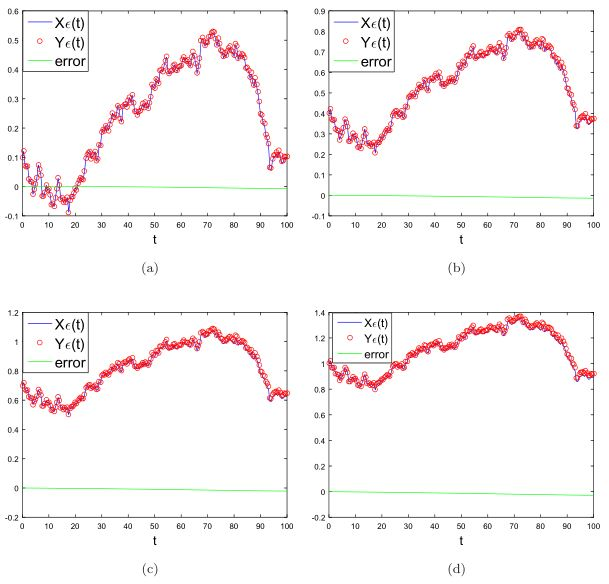
\includegraphics[width=0.80\textwidth]{figure1.JPG}
	\label{figure1}
	\caption{Comparison of the original solution $X_\epsilon(t)$ with the simplified solution $Y_\epsilon(t)$ for Eq.\eqref{5.1}
and \eqref{5.2} with $\epsilon = 0.001$. (a) $X_0 = 0.1, \beta = 0.51$, (b) $X_0 = 0.4, \beta = 0.66,$ (c) $X_0 = 0.7, \alpha = 0.83$,
(d) $X_0 = 1, \alpha = 0.99.$}
\end{figure}

Obviously, the simplified equation \eqref{5.4} is a linear SFDE and it can be easily
solved. All hypotheses in Theorems \ref{4.1} and \ref{4.2} hold, so the solution $Y_\epsilon(t)$ approximates the original solution $X_\epsilon(t)$ to SFDE \eqref{5.3}, and both convergence in
mean sense and probability will be assured.\\

\par In Figure \ref{figure2}, a numerical comparisons between the solutions $X_\epsilon(t)$ and
$Y_\epsilon(t)$ of the original and simplified equations \eqref{5.3} and \eqref{5.4} are presented under
the conditions \\
$X_0 = 0.09, \alpha = 0.55, \epsilon = 0.0001;$\\
$X_0 = 0.15, \alpha = 0.7, \epsilon = 0.0001;$\\
$X_0 = 0.3, \alpha = 0.85, \epsilon = 0.0001;$\\ 
and
$X_0 = 0.5, \alpha = 0.99, \epsilon = 0.0001,$  respectively.\\
\par From Figure \ref{figure2} , a good agreement can be seen between the two solutions
$X_\epsilon(t)$ and $Y_\epsilon(t)$.
\newpage 
\begin{figure}[hp]
	\centering
		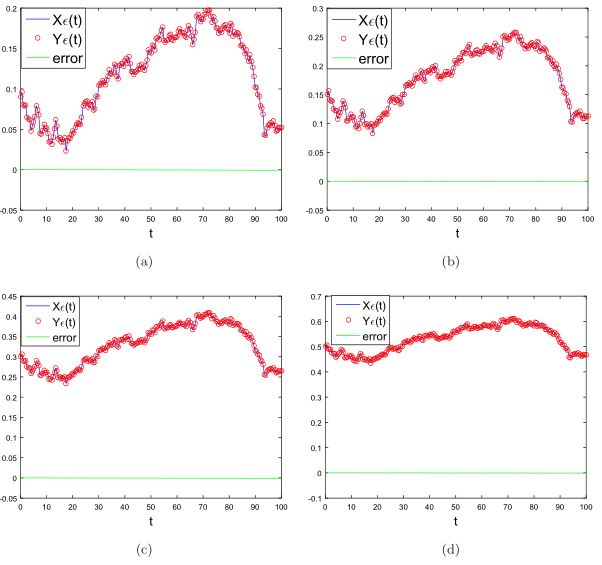
\includegraphics[width=0.80\textwidth]{figure2.JPG}
	\label{figure2}
	\caption{Comparison of the original solution $X_\epsilon(t)$ with the simplified solution $Y_\epsilon(t)$ for Eq.\eqref{5.3}
and \eqref{5.4} with $\epsilon = 0.0001$. (a) $X_0 = 0.09, \beta = 0.55$, (b) $X_0 = 0.15, \beta = 0.7,$ (c) $X_0 = 0.3, \alpha = 0.85$,
(d) $X_0 = 5, \alpha = 0.99.$}
\end{figure}
%there is an image here

\chapter{SUMMARY AND CONCLUSION}
\noindent
\par In this project work, we treated two issues. First, the existence and uniqueness of strong solutions to SFDE's discussed under non-Lipchitz and weakened linear growth condition and this is obtained by Caroth`eodory approximation than an averaging principle for the solutions of SFDE's has proved.
\par This work has considered the connections between the solutions of a standard form and the solutions of averaged systms and prived that under some conditions the solutions of original system in mean square and probability.\\

\par Moreover, a numerical simulation was carried out to show the agreement between the solutions of the original and the simpliied SFDEs.

%
%\begin{equation}\label{}
%
%\end{equation}
%
%\begin{equation}\label{}
%
%\end{equation}
%
%\begin{equation}\label{}
%
%\end{equation}
%
%\begin{equation}\label{}
%
%\end{equation}
%
%\begin{equation}\label{}
%
%\end{equation}
%
%\begin{equation}\label{}
%
%\end{equation}
%
%\begin{equation}\label{}
%
%\end{equation}
%
%\begin{equation}\label{}
%
%\end{equation}
%
%\begin{equation}\label{}
%
%\end{equation}
%
%\begin{equation}\label{}
%
%\end{equation}
%
%\begin{equation}\label{}
%
%\end{equation}
%
%\begin{equation}\label{}
%
%\end{equation}
%
%\begin{equation}\label{}
%
%\end{equation}
%
%\begin{equation}\label{}
%
%\end{equation}
%
%\begin{equation}\label{}
%
%\end{equation}
%
%\begin{equation}\label{}
%
%\end{equation}
%
%\begin{equation}\label{}
%
%\end{equation}
%
















\bibliography{Oluchi799}
\nocite{*}
\bibliographystyle{apacite}
\end{document}